% titlepage-demo.tex
\documentclass{beamer}
\usetheme{Boadilla}
\usepackage{standalone}
\usepackage{multirow}
\usepackage{tikz}
\usepackage{booktabs}
\newcommand{\light}[1]{\textcolor{gray}{#1}}

% highlight the title of the current section
\AtBeginSection[]
{
  \begin{frame}
    \frametitle{Table of Contents}
    \tableofcontents[currentsection]
  \end{frame}
}

\usepackage[absolute,overlay]{textpos} 
\newenvironment{reference}[2]{% 
  \begin{textblock*}{\textwidth}(#1,#2) 
      \footnotesize\it\bgroup\color{red!50!black}}{\egroup\end{textblock*}} 

% items enclosed in square brackets are optional; explanation below
\title[]{Event Detection from Video\\
	 Using Segment-Based Approach}
\subtitle[]{(Final Defense)}
\author[S. Phan]{Sang Phan}
\institute[SOKENDAI]{
  The Graduate University for Advanced Studies (SOKENDAI)\\
  \texttt{plsang@nii.ac.jp}
}
\date[July 2015]{July 22\textsuperscript{nd}, 2015}

\begin{document}

%--- the titlepage frame -------------------------%
\begin{frame}[plain]
  \titlepage
\end{frame}

% % response to committe's requests
\setcounter{framenumber}{0}
% titlepage-demo.tex
\documentclass{beamer}
\usetheme{Boadilla}
\usepackage{multirow}
\usepackage[absolute,overlay]{textpos} 
\newenvironment{reference}[2]{% 
  \begin{textblock*}{\textwidth}(#1,#2) 
      \footnotesize\it\bgroup\color{red!50!black}}{\egroup\end{textblock*}} 



\begin{document}
	
\begin{frame}{Response to Committee's Requests} 	
	\begin{enumerate}
		\item Modify the thesis title.
		\\
		$\rightarrow$ Done. 
		\begin{itemize}
			\item \scriptsize{Old title: Multimedia Event Detection Using Segment-Based Approach.}
			\item New title: Event Detection from Video Using Segment-Based Approach.
		\end{itemize}
		\item Modify chapter titles.
		\\
		$\rightarrow$ Done.
		\begin{itemize}
			\item \scriptsize{Chapter 3: Event Detection Using Segment-based \textbf{Feature Representation}.}
			\item Chapter 4: Event Detection Using Sum-max \textbf{Feature Aggregation}.
			\item Chapter 5: Event Detection Using Event-Driven Multiple Instance \textbf{Learning}.
		\end{itemize}	
		\item Modify the story to cover three contributions.
		\\
		$\rightarrow$ Done (modified in the abstract).
		\item Which challenges are solved by which methods?
		\\
		$\rightarrow$ Done (added in Chapter 6).
		\item Try dynamic pooling (optional).
		\\
		$\rightarrow$ Not yet.
	\end{enumerate}
\end{frame}	


\end{document}
%\setcounter{framenumber}{1}

\begin{frame}
\frametitle{Table of Contents}
\tableofcontents
\end{frame}

\section{Event Detection from Video}



% titlepage-demo.tex
\documentclass{beamer}

\usetheme{Boadilla}


\begin{document}


\begin{frame}[t]{Motivations}
\begin{center}

\includegraphics[width=6cm,height=3cm]{images/MED_overview.png}
\end{center}
\begin{itemize}
\item Massive number of videos are produced every day. 
\begin{itemize}
\item YouTube: 300 hours uploaded per minute, with 3 billion viewers a day.
\end{itemize}
\item Video need to be indexed, searched based on its content.
\item Many applications: 
\begin{itemize}
\item User demands: tutorial videos such as "\textbf{how to make a cake}", "\textbf{how to repair an appliance}".
\item Security purposes: filter out irrelevant content such as "\textbf{how to make a bomb}".

\end{itemize}

\end{itemize}
\end{frame}


%\begin{frame}[t]{Motivation (cont'd)}
%A real world application:	to restrict violent video clips
%	\begin{center}
%		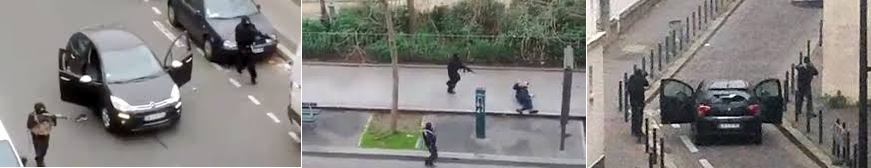
\includegraphics[width=11cm,height=2cm]{images/part1/charlie_hebdo_attacks.png}
%		\\
%		Footage of the Charlie Hebdo Attack (Paris - Jan 2015)
%	\end{center}
%	\begin{center}
%		
\includegraphics[width=6cm,height=3.5cm]{images/part1/facebook.png}
%		\\
%		Facebook has begun placing warnings over videos posted to its site
%	\end{center}
%\end{frame}

\begin{frame}[t]{Motivations (cont'd)}
A real world application: \textbf{detect shoplifting} (``manbiki'').

\begin{itemize}
	\item Jan, 2015: National manhunt in Japan for a YouTuber who allegedly stole...snacks [Mainichi News].
\end{itemize}
	\begin{center}
		
\includegraphics[width=11cm,height=2cm]{images/part1/snacks.png}
		\\
		The footage shows that he's stolen many things. 
	\end{center}
\begin{itemize}
	\item How can the police know? 
	\begin{itemize}
\item Because he has been uploading clips of his alleged thefts.
	\end{itemize}
	\item Can it be \textbf{automatically} detected by security cameras? 
\end{itemize}
\begin{tikzpicture}[remember picture,overlay]  
\node [xshift=-1.3cm,yshift=-7.5cm] at (current page.north east)
{
\includegraphics[width=2cm,height=2cm]{images/part1/conan.jpg}};
\end{tikzpicture}

\end{frame}


\begin{frame}[t]{Complex Event}
	\begin{definition} 
		\begin{itemize}
		\item is a complex activity occurring at a specific place and time;
		\item involves people interacting with other people and/or objects;
		\item consists of a number of human actions, processes and activities.
		\end{itemize}
	\end{definition}
	\begin{center}
	\begin{figure}
		\centering
		\begin{minipage}{.3\textwidth}
			\centering
			
\includegraphics[width=1\linewidth]{images/part1/shoplifting1.jpg}
			\\
			\tiny{Pick up an item}
		\end{minipage}%
		\begin{minipage}{.3\textwidth}
			\centering
			
\includegraphics[width=1\linewidth]{images/part1/shoplifting2.jpg}
			\\
			\tiny{Keep it in a hidden place}
		\end{minipage}
		\begin{minipage}{.3\textwidth}
			\centering
			
\includegraphics[width=1\linewidth]{images/part1/shoplifting3.jpg}
			\\
			\tiny{Get out successfuly}
		\end{minipage}
\footnotesize{Sequence of actions in the shoplifting event.}
	\end{figure}

	\end{center}
\small{Compared to \textbf{single action} detection [KTH dataset]}
	\begin{center}
		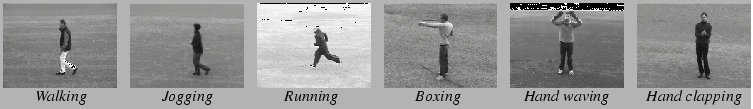
\includegraphics[width=11cm,height=1.6cm]{images/part1/kth.png}
	\end{center}
\end{frame}


\begin{frame}[t]{Event Detection from Video}
In 2010 TRECVID proposed Multimedia Event Detection (MED) task.
\begin{definition}
\begin{itemize}
\item Given: An event kit which consists of an event name, definition, explication + video example.
\item Wanted: A system that can search for this event through the large set of videos with reasonable accuracy and speed.
\end{itemize}
\end{definition}
\begin{center}
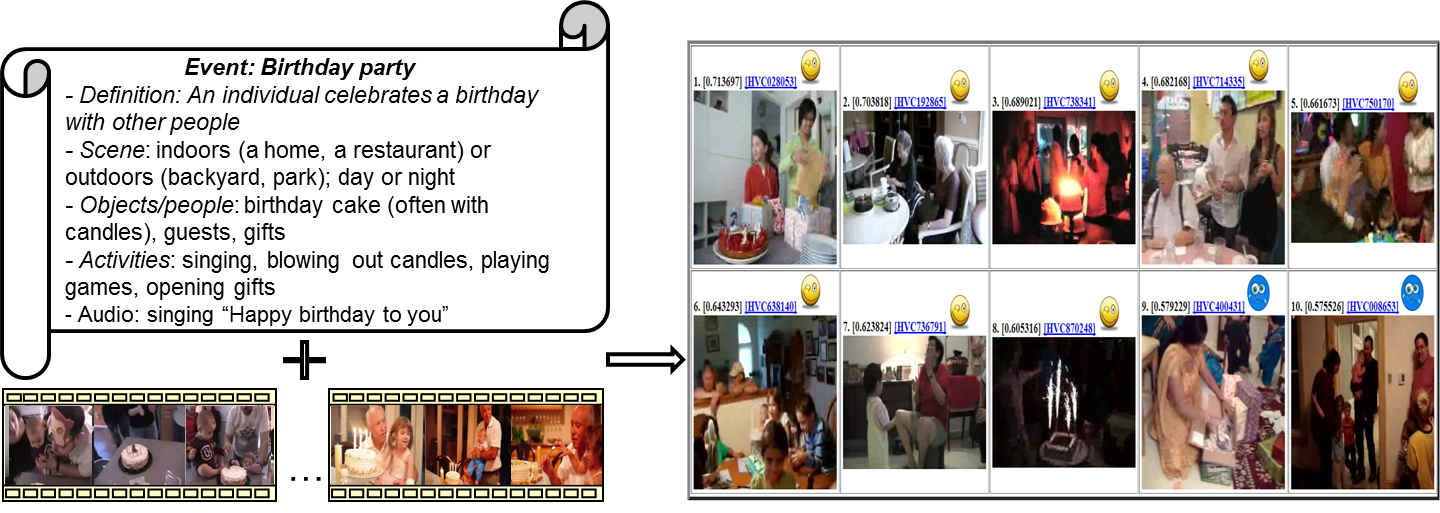
\includegraphics[width=12cm,height=4cm]{images/med_definition.png}
\end{center}


\end{frame}

\begin{frame}[t]{Challenges of Event Detection from Video}
	\begin{itemize}
		\item \textbf{Large content variation}: the diversity of complex
		event is very high.
	\end{itemize}
\begin{center}
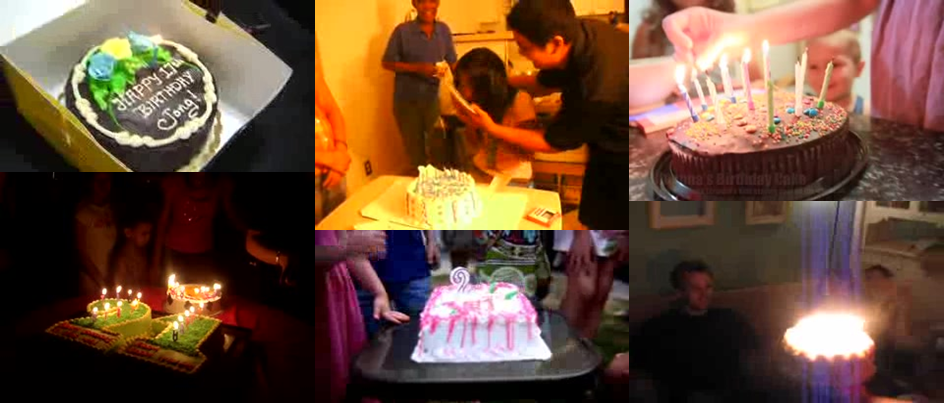
\includegraphics[width=10cm,height=4.5cm]{images/part1/largevariation.png}
\\
The large variation of \textit{birthday cake} in the ``birthday party'' event.
\end{center}
\end{frame}


\begin{frame}[t]{Challenges of Event Detection from Video (cont'd)}
	\begin{itemize}
		\item \textbf{Uncontrolled capturing conditions}: different time, location, clutter in the environment, camera motion $\rightarrow$ can contain irrelevant information to the event of interest.
	\end{itemize}
	\begin{center}
		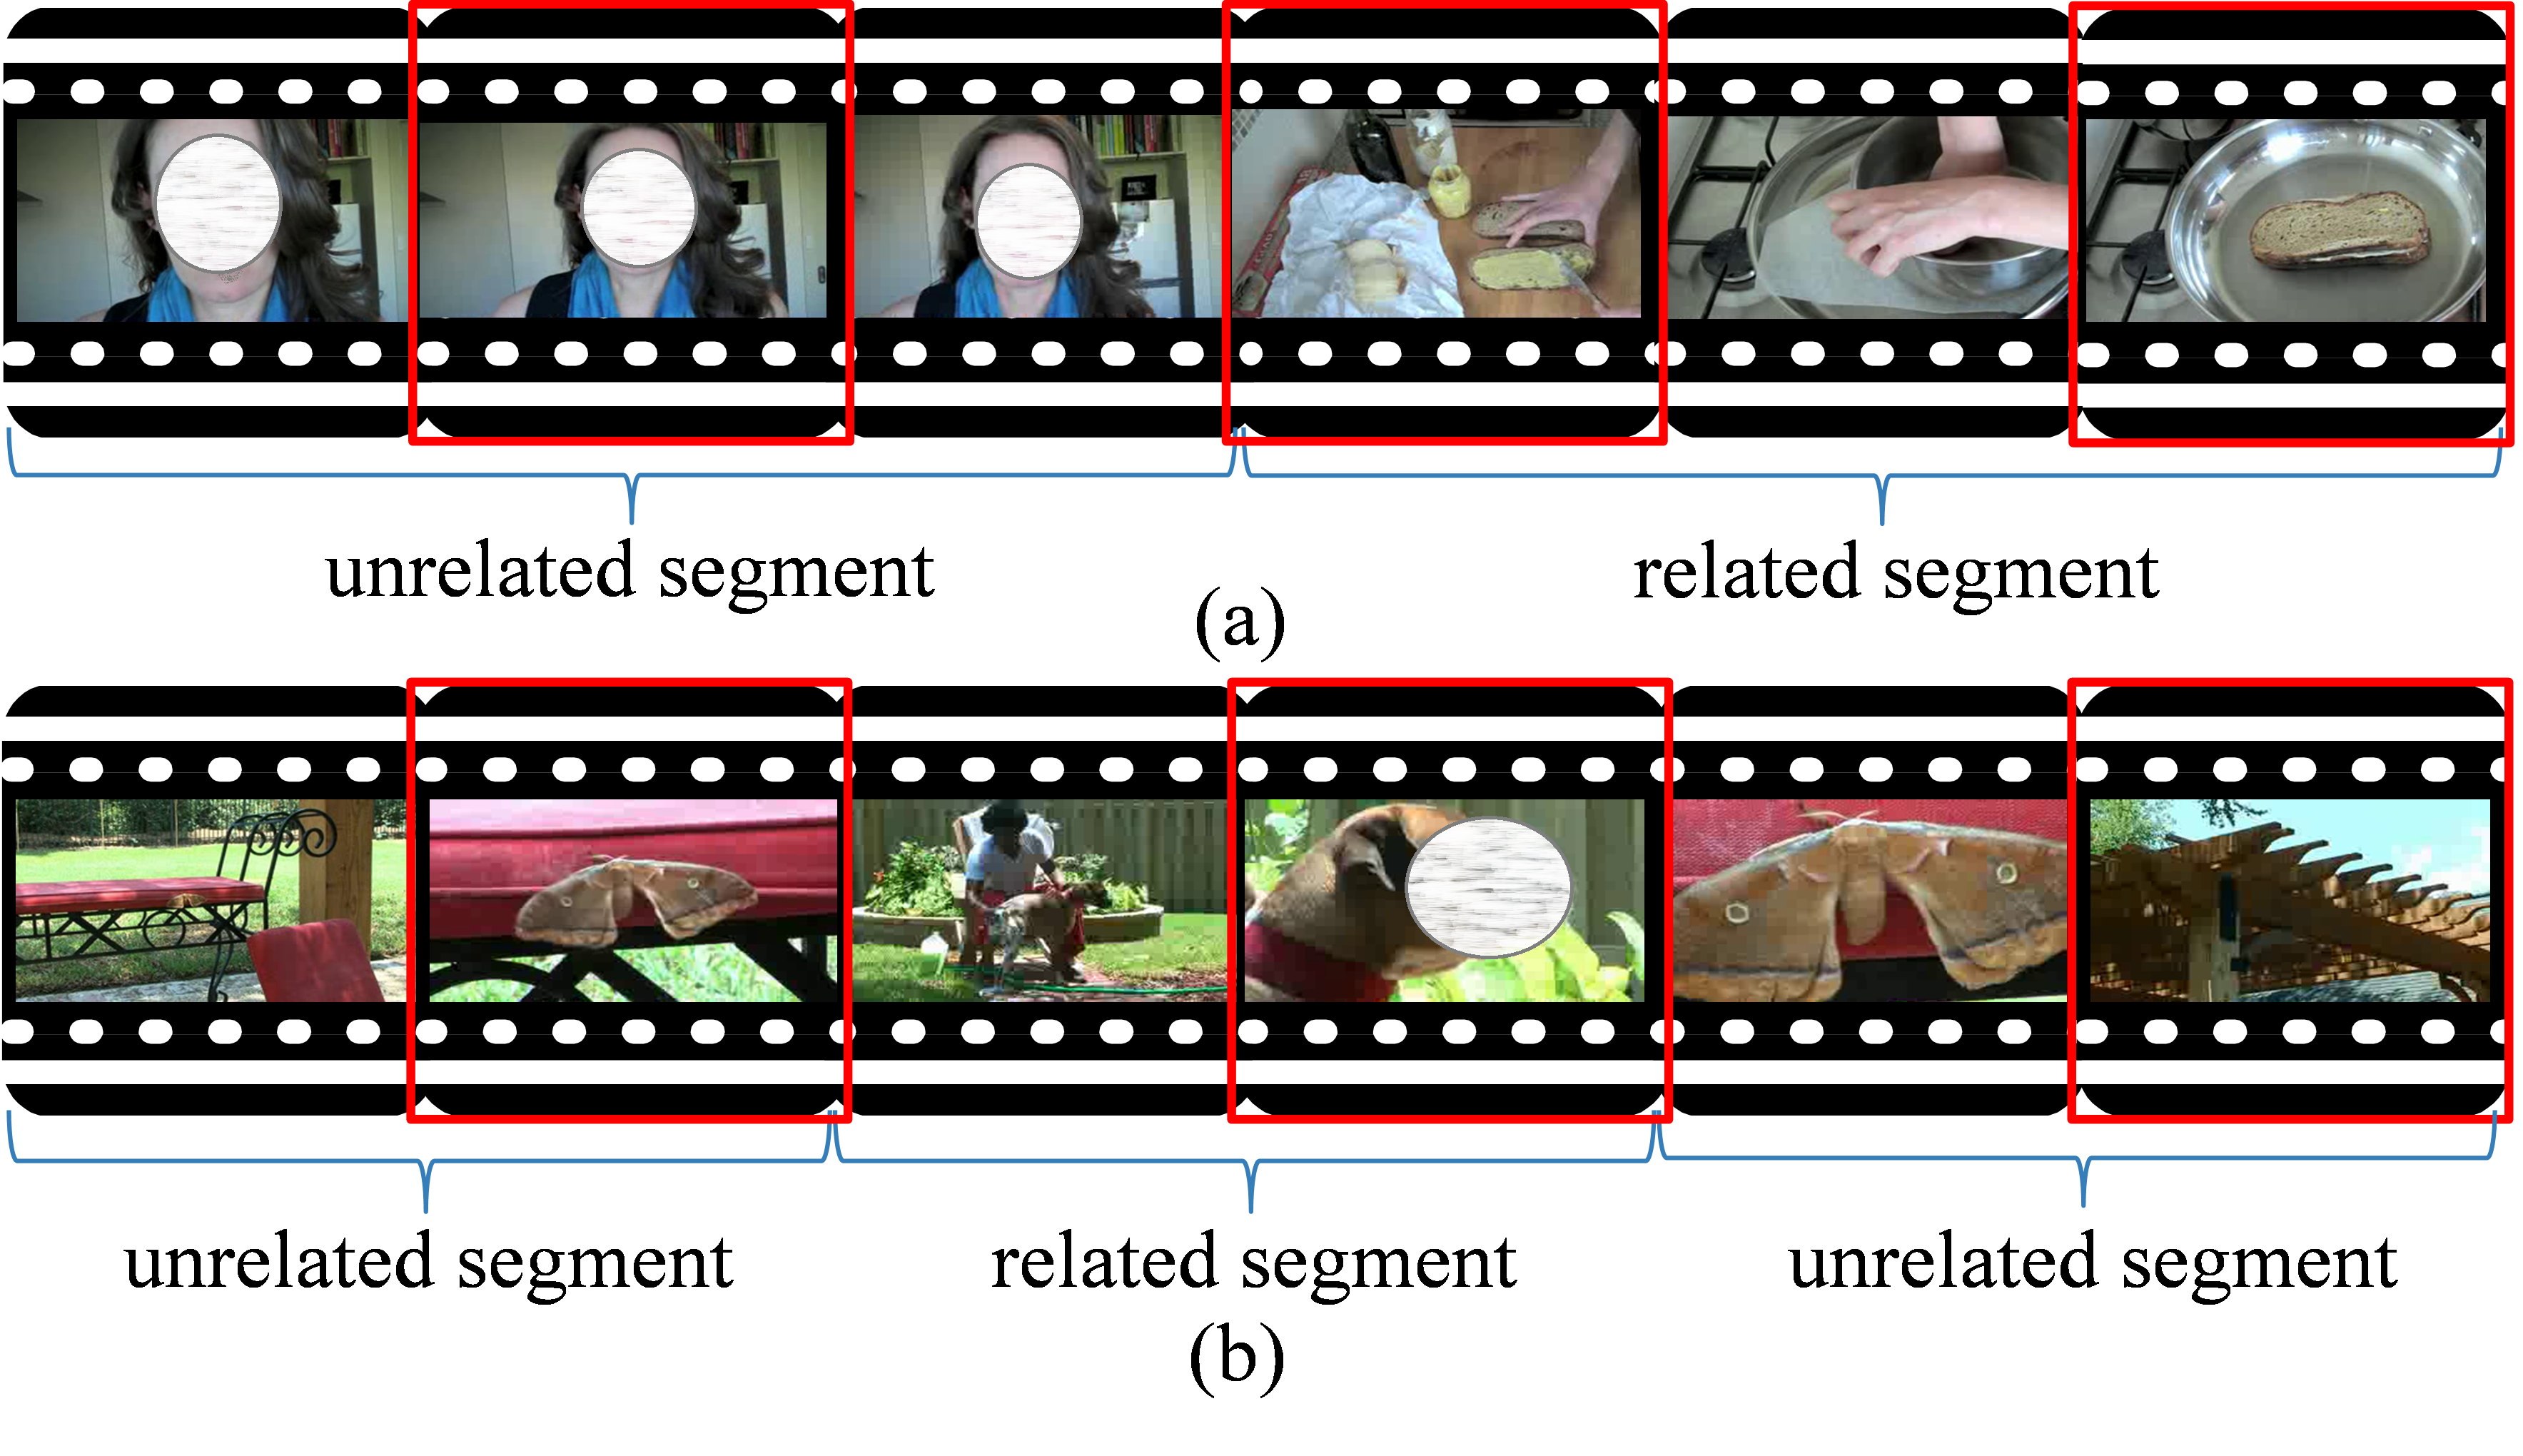
\includegraphics[width=10cm,height=5cm]{images/part1/uncontrolled.png}
		\\
		\footnotesize{(a) Example video for ``making a sandwich'' event: the related segment appears after a self-cam segment (unrelated); (b) example video for ``grooming an animal'' event: related segment is sandwiched between two unrelated segments.}
	\end{center}
	
\end{frame}


\begin{frame}[t]{Challenges of Event Detection from Video (cont'd)}
	
	\begin{itemize}
		\item Presence of \textbf{near-miss} (related) videos.
			\begin{itemize}
	\item closely related to the event but it lacks critical evidences to be a positive event instance.
			\end{itemize}
	\end{itemize}
	
	\begin{center}
		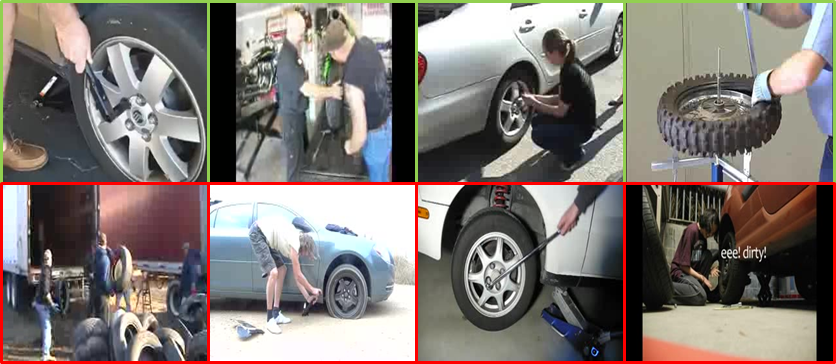
\includegraphics[width=10cm,height=4.5cm]{images/part1/nearmiss.png}
		\\
			\footnotesize{Example of \textit{near-miss} videos for ``Changing a vehicle tire'' event (2\textsuperscript{nd} row).}
	\end{center}
\end{frame}

\begin{frame}[t]{Challenges of Event Detection from Video (cont'd)}
\begin{itemize}
\item Large scale video archives
\end{itemize}
%\begin{tabular}{ | p{2cm} | p{2.5cm} | p{3cm} | p{3cm} | }
%\hline
%	Dataset & MED 2010 & MED 2011 & MED 2012  \\ \hline
%	Number of test events & \textbf{3} (Assembling a shelter, Batting a run, Making a cake) & \textbf{10} (Birthday party, Changing a vehicle tire, Flashmob gathering, etc) & \textbf{20} (Cleaning an appliance, Dog show, Marriage proposal, etc)  \\ \hline
%	Number of videos & \textbf{3,468} (1,744 dev videos and 1,724 test videos) & \textbf{45,000} (13,200 dev videos and 31,800 test videos) & \textbf{156,000} videos (58,000 dev videos and 98,000 test videos) \\ \hline
%	Number of background videos & \textbf{1,500} for dev and \textbf{1,500} for test & \textbf{10,000} for dev and \textbf{28,000} for test & \textbf{10,000} for dev and \textbf{95,000} for test \\ \hline
%	Hours of video & \textbf{110} & \textbf{1,400} & \textbf{4,850} \\ \hline
%\end{tabular}

\begin{table}[h]
	\centering
		Number of videos in the TRECVID MED collection up to 2014.
	\scriptsize
	\begin{tabular}{@{}|c|l|c|c|@{}}
		\toprule
		\multicolumn{2}{|c|}{Set}                                                                         & Number of video clips & Video duration (hours) \\ \midrule
		\multirow{3}{*}{\begin{tabular}[c]{@{}c@{}}Development\\ Data\end{tabular}}    & RESEARCH         & 10,000                & 314                    \\ \cmidrule(l){2-4} 
		& 10 Event Kits    & 1,400                 & 74                     \\ \cmidrule(l){2-4} 
		& Transcription    & 1,500                 & 45                     \\ \midrule
		\multirow{2}{*}{\begin{tabular}[c]{@{}c@{}}Event\\ Training Data\end{tabular}} & Event Background & 5,000                 & 146                    \\ \cmidrule(l){2-4} 
		& 40 Event Kits    & 6,000                 & 270                    \\ \midrule
		\multirow{2}{*}{Test Data}                                                     & MEDTest          & 27,000                & 849                    \\ \cmidrule(l){2-4} 
		& KindredTest      & 14,500                & 687                    \\ \midrule
		\multirow{2}{*}{Evaluation Data}                                               & MED14Eval-Full   & 198,000               & 7,580                  \\ \cmidrule(l){2-4} 
		& MED14Eval-Sub    & 33,000                & 1,244                  \\ \midrule
		\multicolumn{2}{|c|}{\textbf{Total}}                                                                       & \textbf{244,000}               & \textbf{9,911}                  \\ \bottomrule \bottomrule
		
				\multicolumn{2}{|c|}{\textbf{THUMOS14 (largest action dataset)}}                                                                       & \textbf{13,000}               & \textbf{254}                  \\ \bottomrule
	\end{tabular}
	\label{c2_dataset}
\end{table}

\end{frame}


\begin{frame}[t]{Target Challenge \& Research Direction}
	\begin{itemize}
		\item Target challenge: \textit{\textbf{Uncontrolled capturing conditions}} 
			\begin{itemize}
				
\item contains irrelevant information to the event of interest.
\item differentiates real video from studio/controlled-capturing video.
		 	\end{itemize}
		\item Research direction: Decompose the video into sub-sequences and study event detection methods from these sub-sequences.
	\end{itemize}
	\begin{center}
		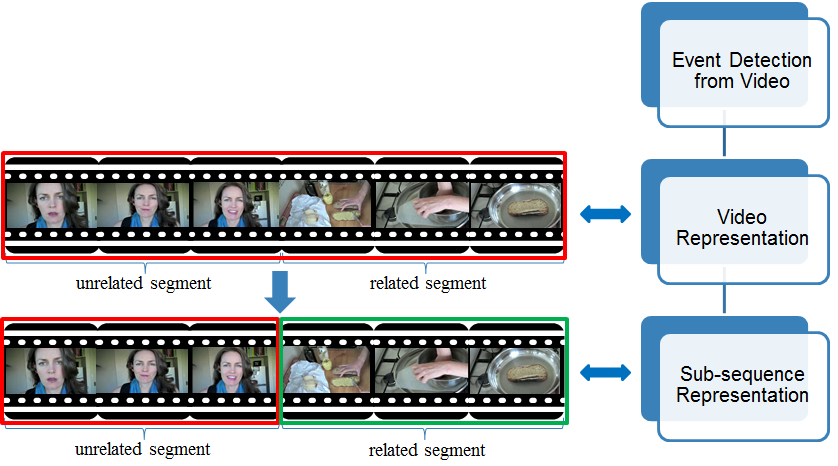
\includegraphics[width=10cm,height=5.5cm]{images/part1/mainchallenge.png}
		\\
		\footnotesize{}
	\end{center}
	
\end{frame}


\begin{frame}[t]{Contributions}
	
	\begin{enumerate}
		\item Segment-based \textbf{Representation} (SB)
		\begin{itemize}
			\item Investigate different strategies to \\
			decompose a video into segments.
			\item Study the optimal segment length.
		\end{itemize}
		\item Sum-Max Video \textbf{Aggregation} (SM)
		\begin{itemize}
			\item An efficient method to aggregate\\
			local features into video feature \\
			representation.
		\end{itemize}
		\item Event-driven Multiple Instance \\
				\textbf{Learning} (EDMIL)
		\begin{itemize}
			\item A method to leverage the event\\
			 description to learn key evidences \\
			 for complex event detection.
		\end{itemize}
	\end{enumerate}
	
\begin{tikzpicture}[remember picture,overlay]  
\node [xshift=-3cm,yshift=-4.5cm] at (current page.north east)
{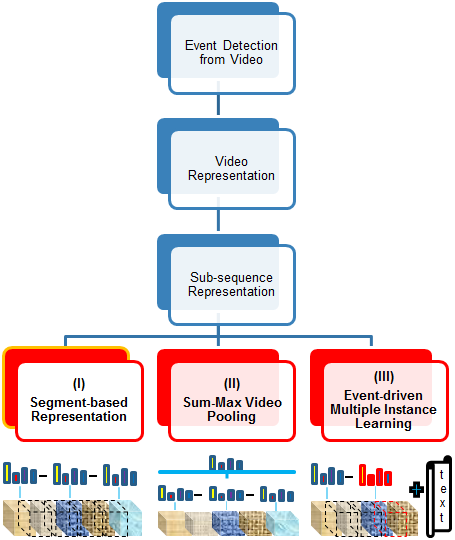
\includegraphics[width=5cm,height=7.5cm]{images/part1/contribution2.png}};
\end{tikzpicture}

\end{frame}

\end{document}


\section{Segment-based Feature Representation}


% titlepage-demo.tex
\documentclass{beamer}
\usetheme{Boadilla}
\usepackage{multirow}
\usepackage[absolute,overlay]{textpos} 
\newenvironment{reference}[2]{% 
  \begin{textblock*}{\textwidth}(#1,#2) 
      \footnotesize\it\bgroup\color{red!50!black}}{\egroup\end{textblock*}} 

\begin{document}

\begin{frame}[t]{How to Detect Event in Video?}
	\begin{itemize}
		\item State-of-the-art systems [Jiang-TRECVID2010], [Natarajan-TRECVID2011] (\textbf{best systems} in TRECVID MED 2010 and 2011)
	\end{itemize}
	
	\begin{center}
		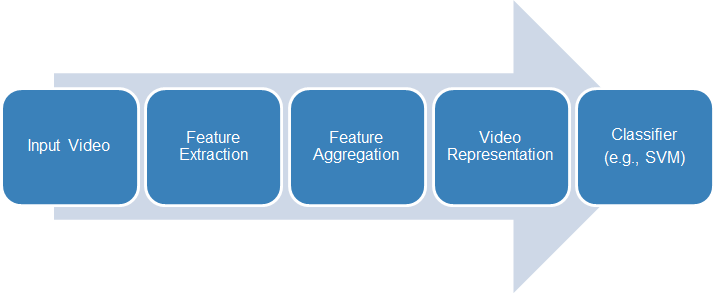
\includegraphics[width=10cm,height=4cm]{images/part2/standardapproach.png}
	\end{center}
	
	\textbf{Problem}: Neutralize the contribution of each part of the whole video. 
	\begin{itemize}
		\item In fact, the clues to determine an event often appear in a small segment.
	\end{itemize}
	
\end{frame}

\begin{frame}[t]{How to Detect Event in Small Segments of Video?}
		\begin{itemize}
\item Straightforward solutions: Split the videos into segments and detect event in these small segments. 
	\begin{itemize}
		\item $[$Niebles-ECCV2010] and [Gaidon-CVPR2011] model activities as sequences of atomic actions using semantic attributes.
		\item $[$Tang-CVPR2012] model the key segments and segment duration as latent variables and solve using a variant of HMM.
		\item $[$Vahdat-ICCV2013] Localize the most salient evidences using latent SVM. 
		\item $[$Lai-CVPR2014] Detect key instances in video based on a variant of Multiple Instance Learning. 
	\end{itemize}

\item Limitations
	\begin{itemize}
		\item Segmentation of activities into predefined atomic
		actions and annotation of these atomic actions are available.
		\item Video sequences are precisely cropped with activities of interest.
		\item Use fixed length segment. 
	\end{itemize}
			\end{itemize}
	$\rightarrow$ \textbf{We do not know what is the optimal segment length when splitting the whole video!}
	
\end{frame}

%\begin{frame}[t]{Video-based Approach}
%\begin{itemize}
%\item Features are computed over the whole video
%\item One representation for each video
%\end{itemize}

%\begin{center}
%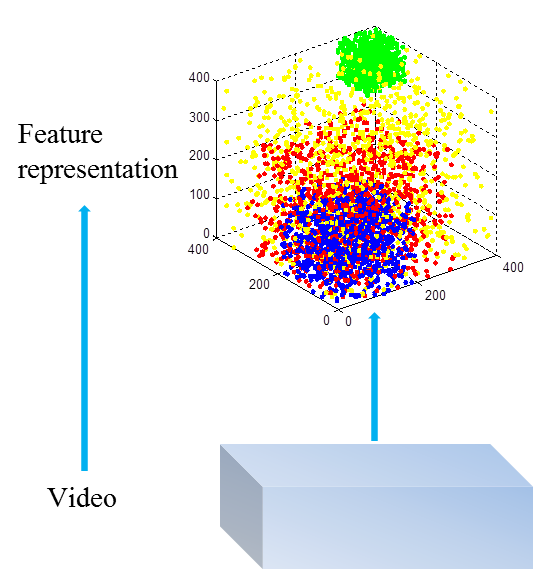
\includegraphics[width=5cm,height=4.5cm]{images/video_based.png}
%\end{center}

%\begin{itemize}
%\item Used by best MED'10 system (Columbia University)
%\item Used by best MED'11 system (BBN VISER)
%\end{itemize}

%\textbf{Specific problem}: The clues to determine an event can reside within a small segment.
%\end{frame}

\begin{frame}{Our Segment-based Approach} 
\begin{itemize}
	\item We investigate different strategies to split the videos in segments.
	\item We study the optimal segment length.
\end{itemize}
%\bigskip
\begin{columns}
  \begin{column}{0.3\textwidth}
    \centerline{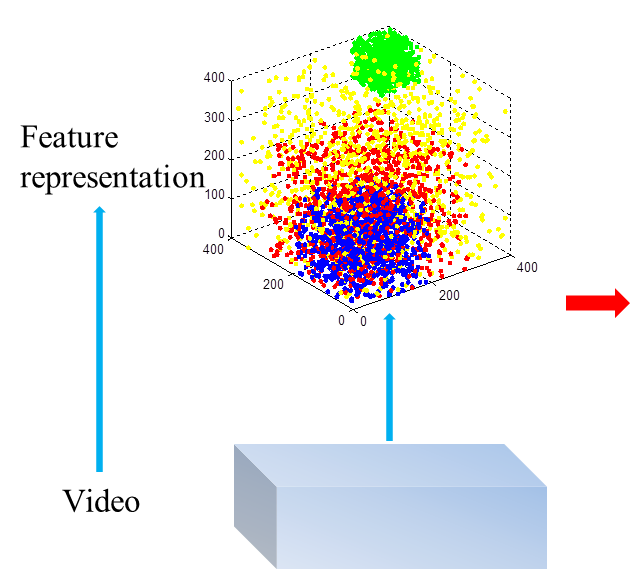
\includegraphics[width=1\textwidth]{images/video_based2.png}}
    (a) The video-based approach
  \end{column}

  \begin{column}{0.7\textwidth}
    \centerline{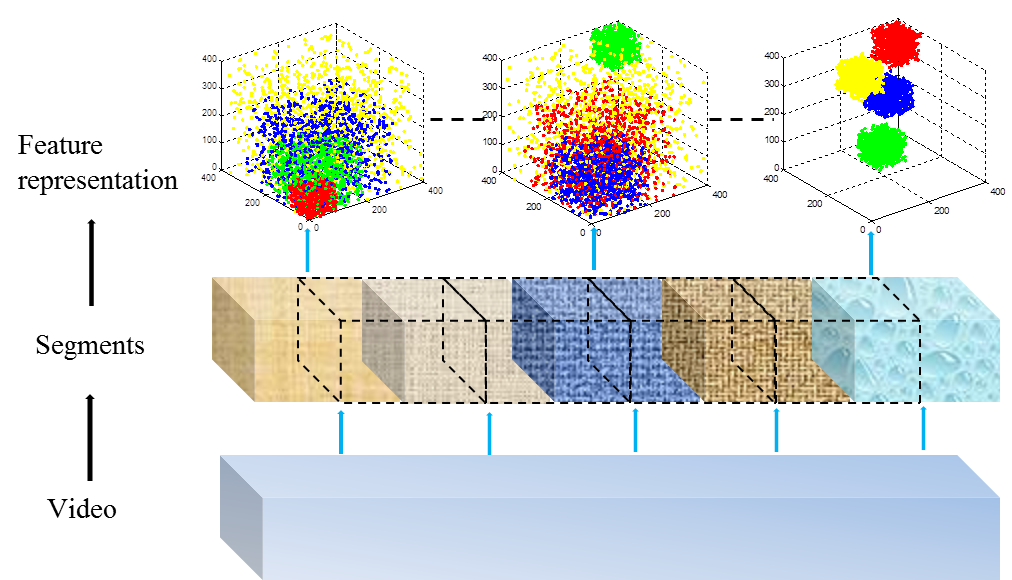
\includegraphics[width=1\textwidth]{images/segment_based.png}}
    (b) \textbf{Our proposed segment-based approach}
  \end{column}
\end{columns}
\bigskip
 
  
\end{frame}

\begin{frame}[t]{Our Segment-based Approach}
\textbf{How to select the segment length?}
\begin{itemize}
\item Non-overlapping
\begin{itemize}
	\item Uniform sampling
	\item Segment length: 30, 60, 90, 120, 200, 400 seconds 
	\item Compare with the video-based approach (using the whole video)
\end{itemize}
\item Overlapping sampling
	\begin{itemize}
	\item Uniform sampling, 50\% overlapping
	\item Segment length: 30, 60, 90, 120, 200, 400 seconds 
	\item Compare with the video-based approach (using the whole video)
	\end{itemize}
\item Segment sampling based on shot boundary detection
	\begin{itemize}
	\item Take into account the boundary information of each segment
	\item Employ the technique proposed by [Guimaraes et al. - 2003]
	\end{itemize}
	
\begin{reference}{4mm}{85mm}
Guimaraes, S.J.F., Couprie, M., Araujo, A.d.A., Leite, N.J: Video segmentation based on 2d image analysis. Pattern Recognition Letters, 2003, 24(7), 947–957.
\end{reference} 
	
\end{itemize}

\end{frame}

\begin{frame}[t]{Evaluation Framework}
\begin{center}
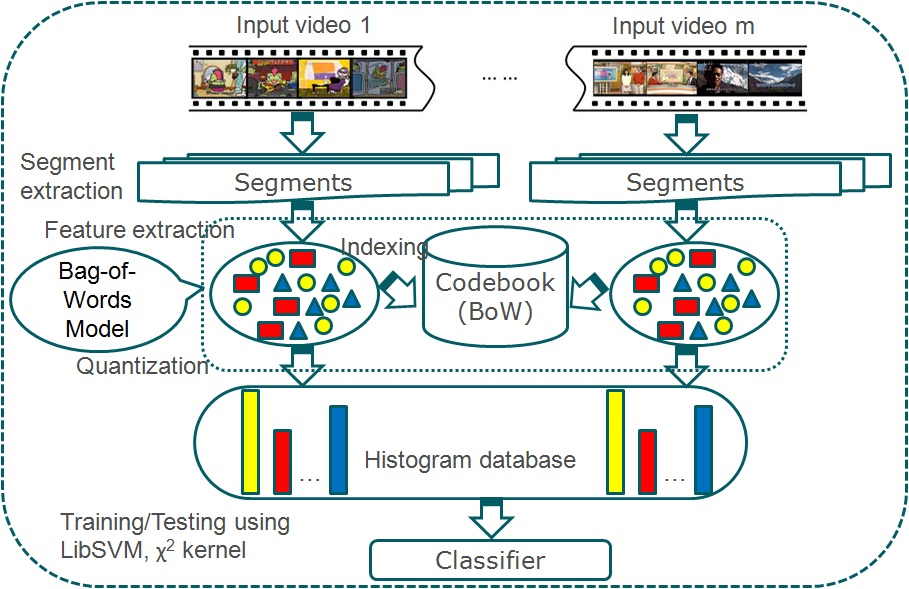
\includegraphics[width=10cm,height=6cm]{images/framework2.jpg}
\\
Evaluation framework for our event detection system.
\end{center}

\end{frame}

\begin{frame}{Experimental Setup} 	
	\begin{itemize}
		\item Dataset
		
		\begin{table}[h]
			\tiny
			\begin{tabular}{@{}|l|c|c|c|c|c|@{}}
				\toprule
				\multicolumn{1}{|c|}{Dataset} & No. Event & No. Train Videos & No. Test Videos & Total Videos & Total Hours \\ \midrule
				MED2010 & 3 & 1,744 & 1,724 & 3,468 & 110 hours \\ \midrule
				MED2011 & 10 & 12,590 & 31,822 & 33,153 & 1,400 hours \\ \midrule
				\light{MED2012} & \light{25} & \light{3,878} & \light{1,938} & \light{5,816} & \light{250 hours} \\ \bottomrule
			\end{tabular}
		\end{table}
		
		\item Feature: Dense Trajectories, MBH descriptor [Wang-CVPR2011] 	
		\item Feature encoding: Bag-of-words model, 4000 codewords.
		\item Learning: ${\chi}^{2}$ SVM.
	\end{itemize}
	
\end{frame}	

\begin{frame}{Result: Non-Overlapping vs. Overlapping Sampling} 

\bigskip

\begin{columns}
  \begin{column}{0.5\textwidth}
    \centerline{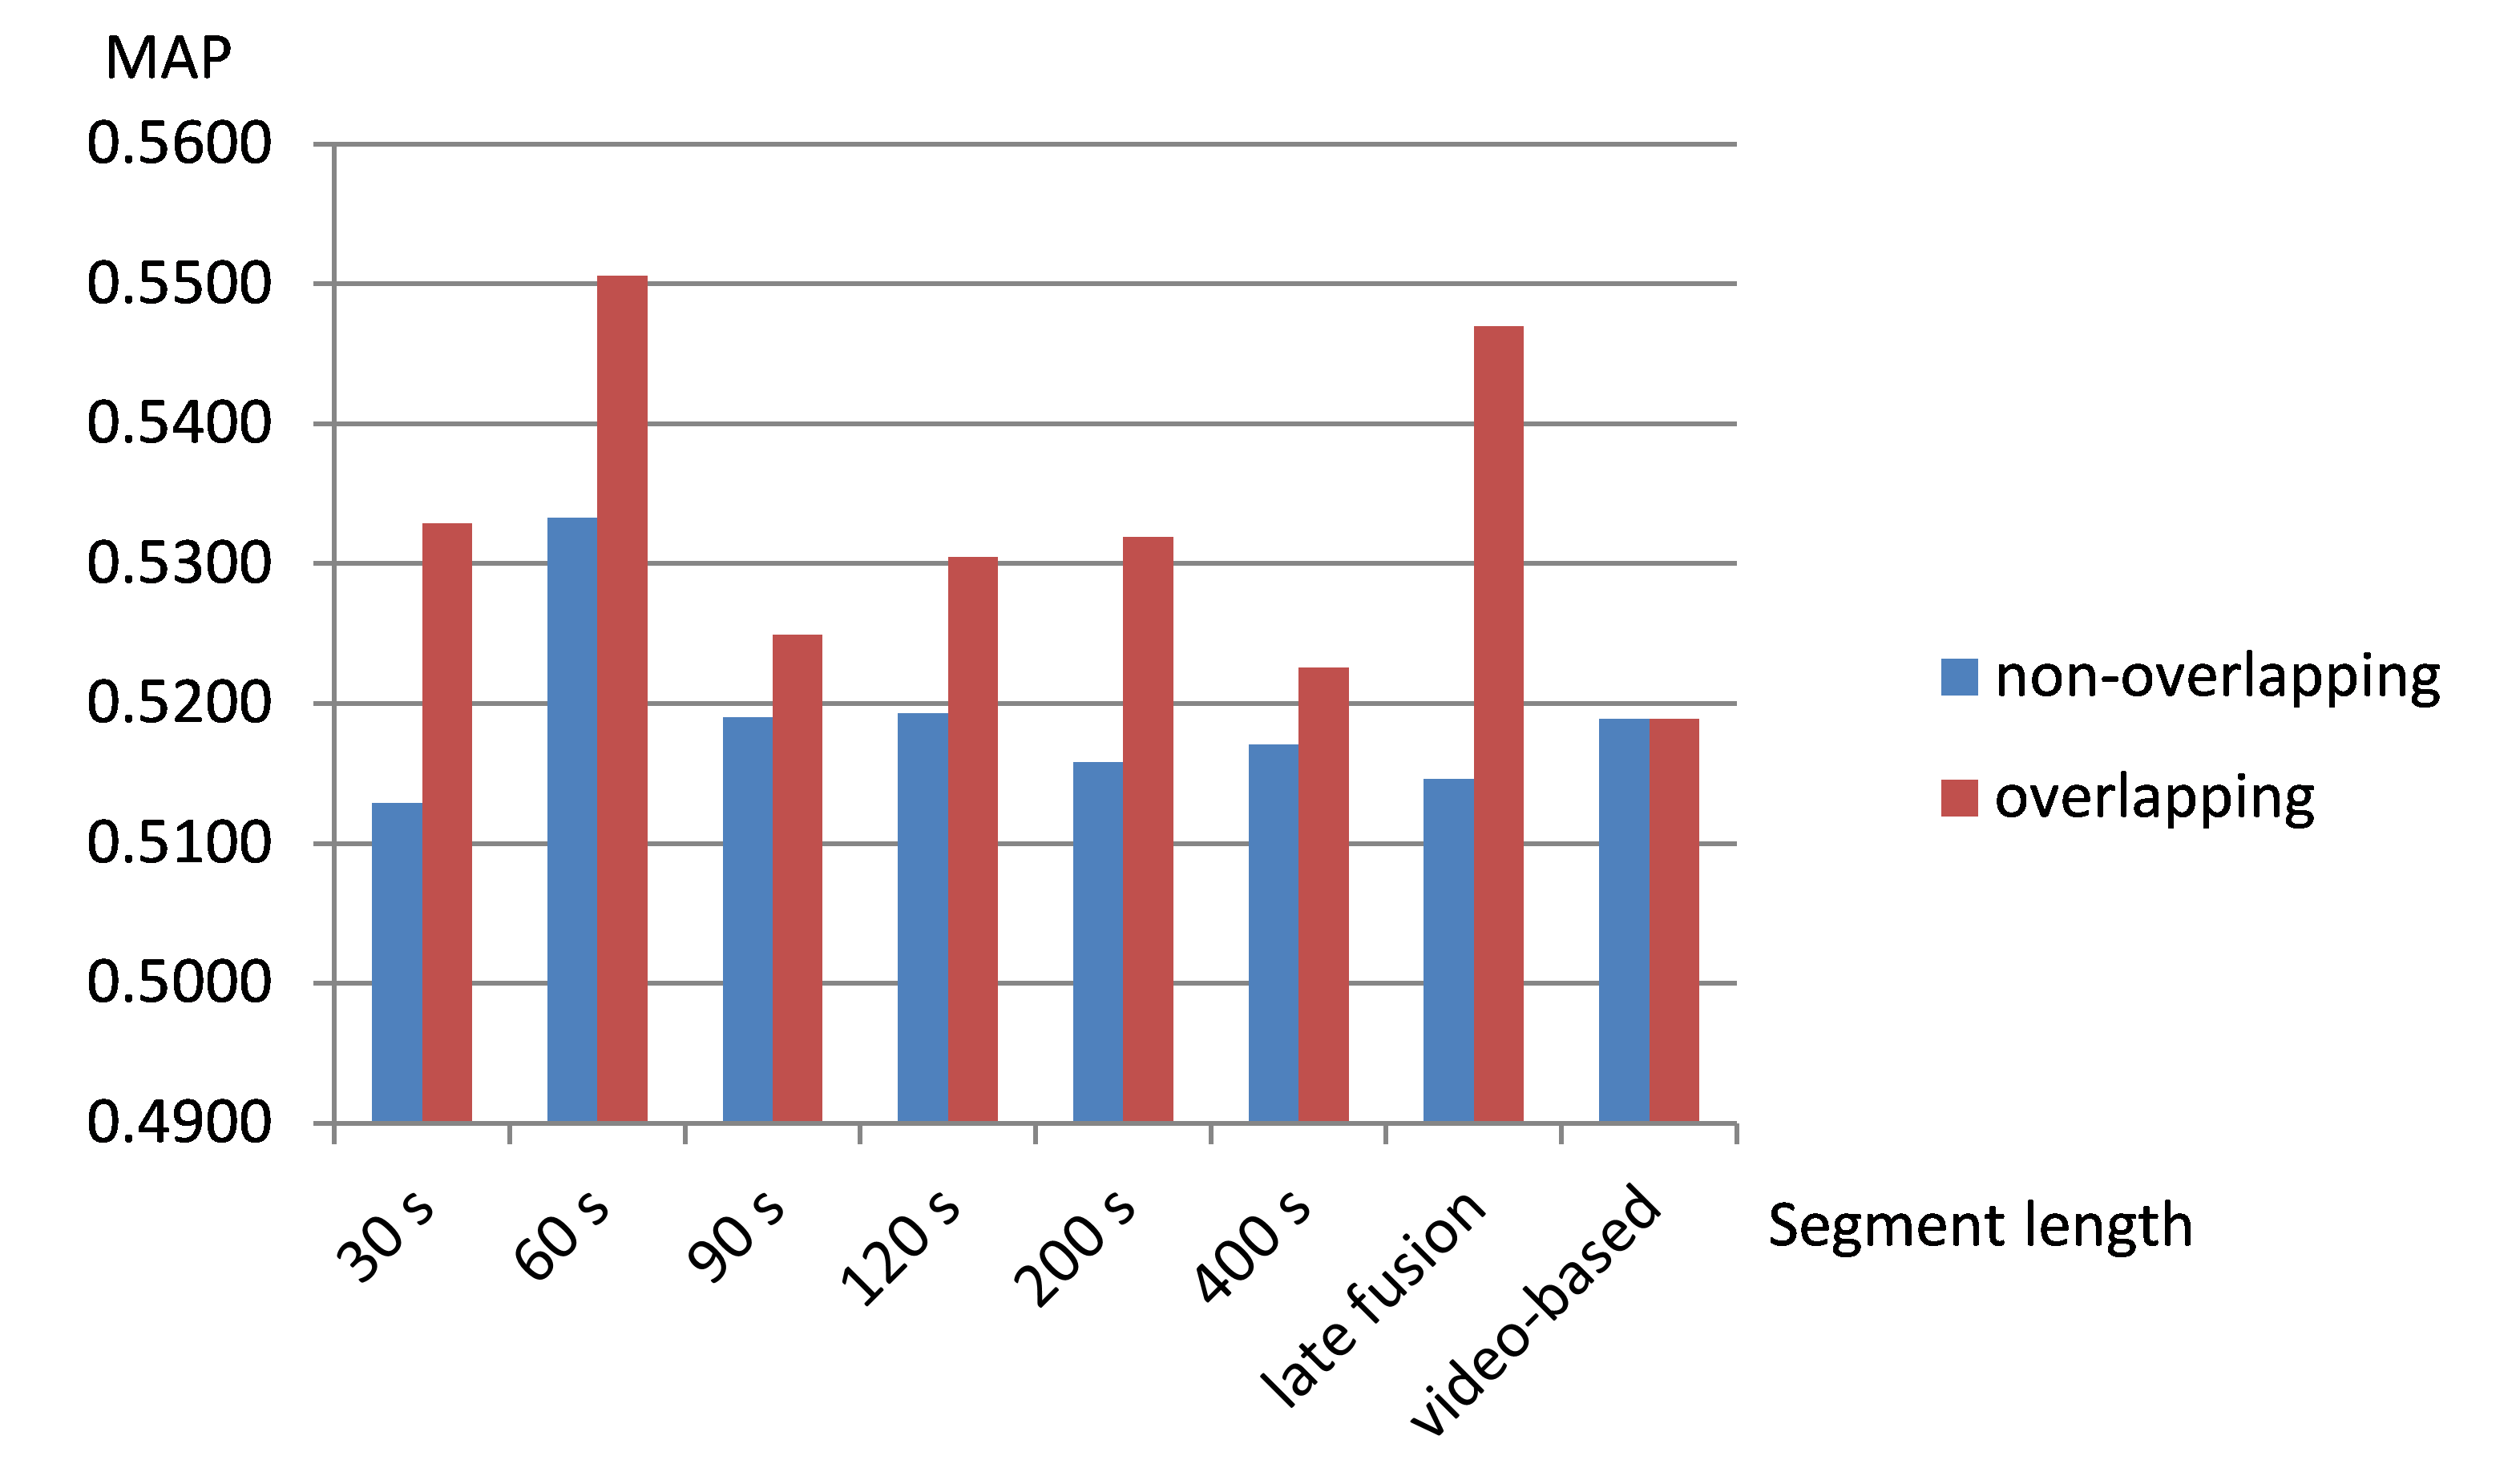
\includegraphics[width=1\textwidth]{images/med10_result.png}}
    (b) On the MED 2010 dataset
  \end{column}

  \begin{column}{0.5\textwidth}
    \centerline{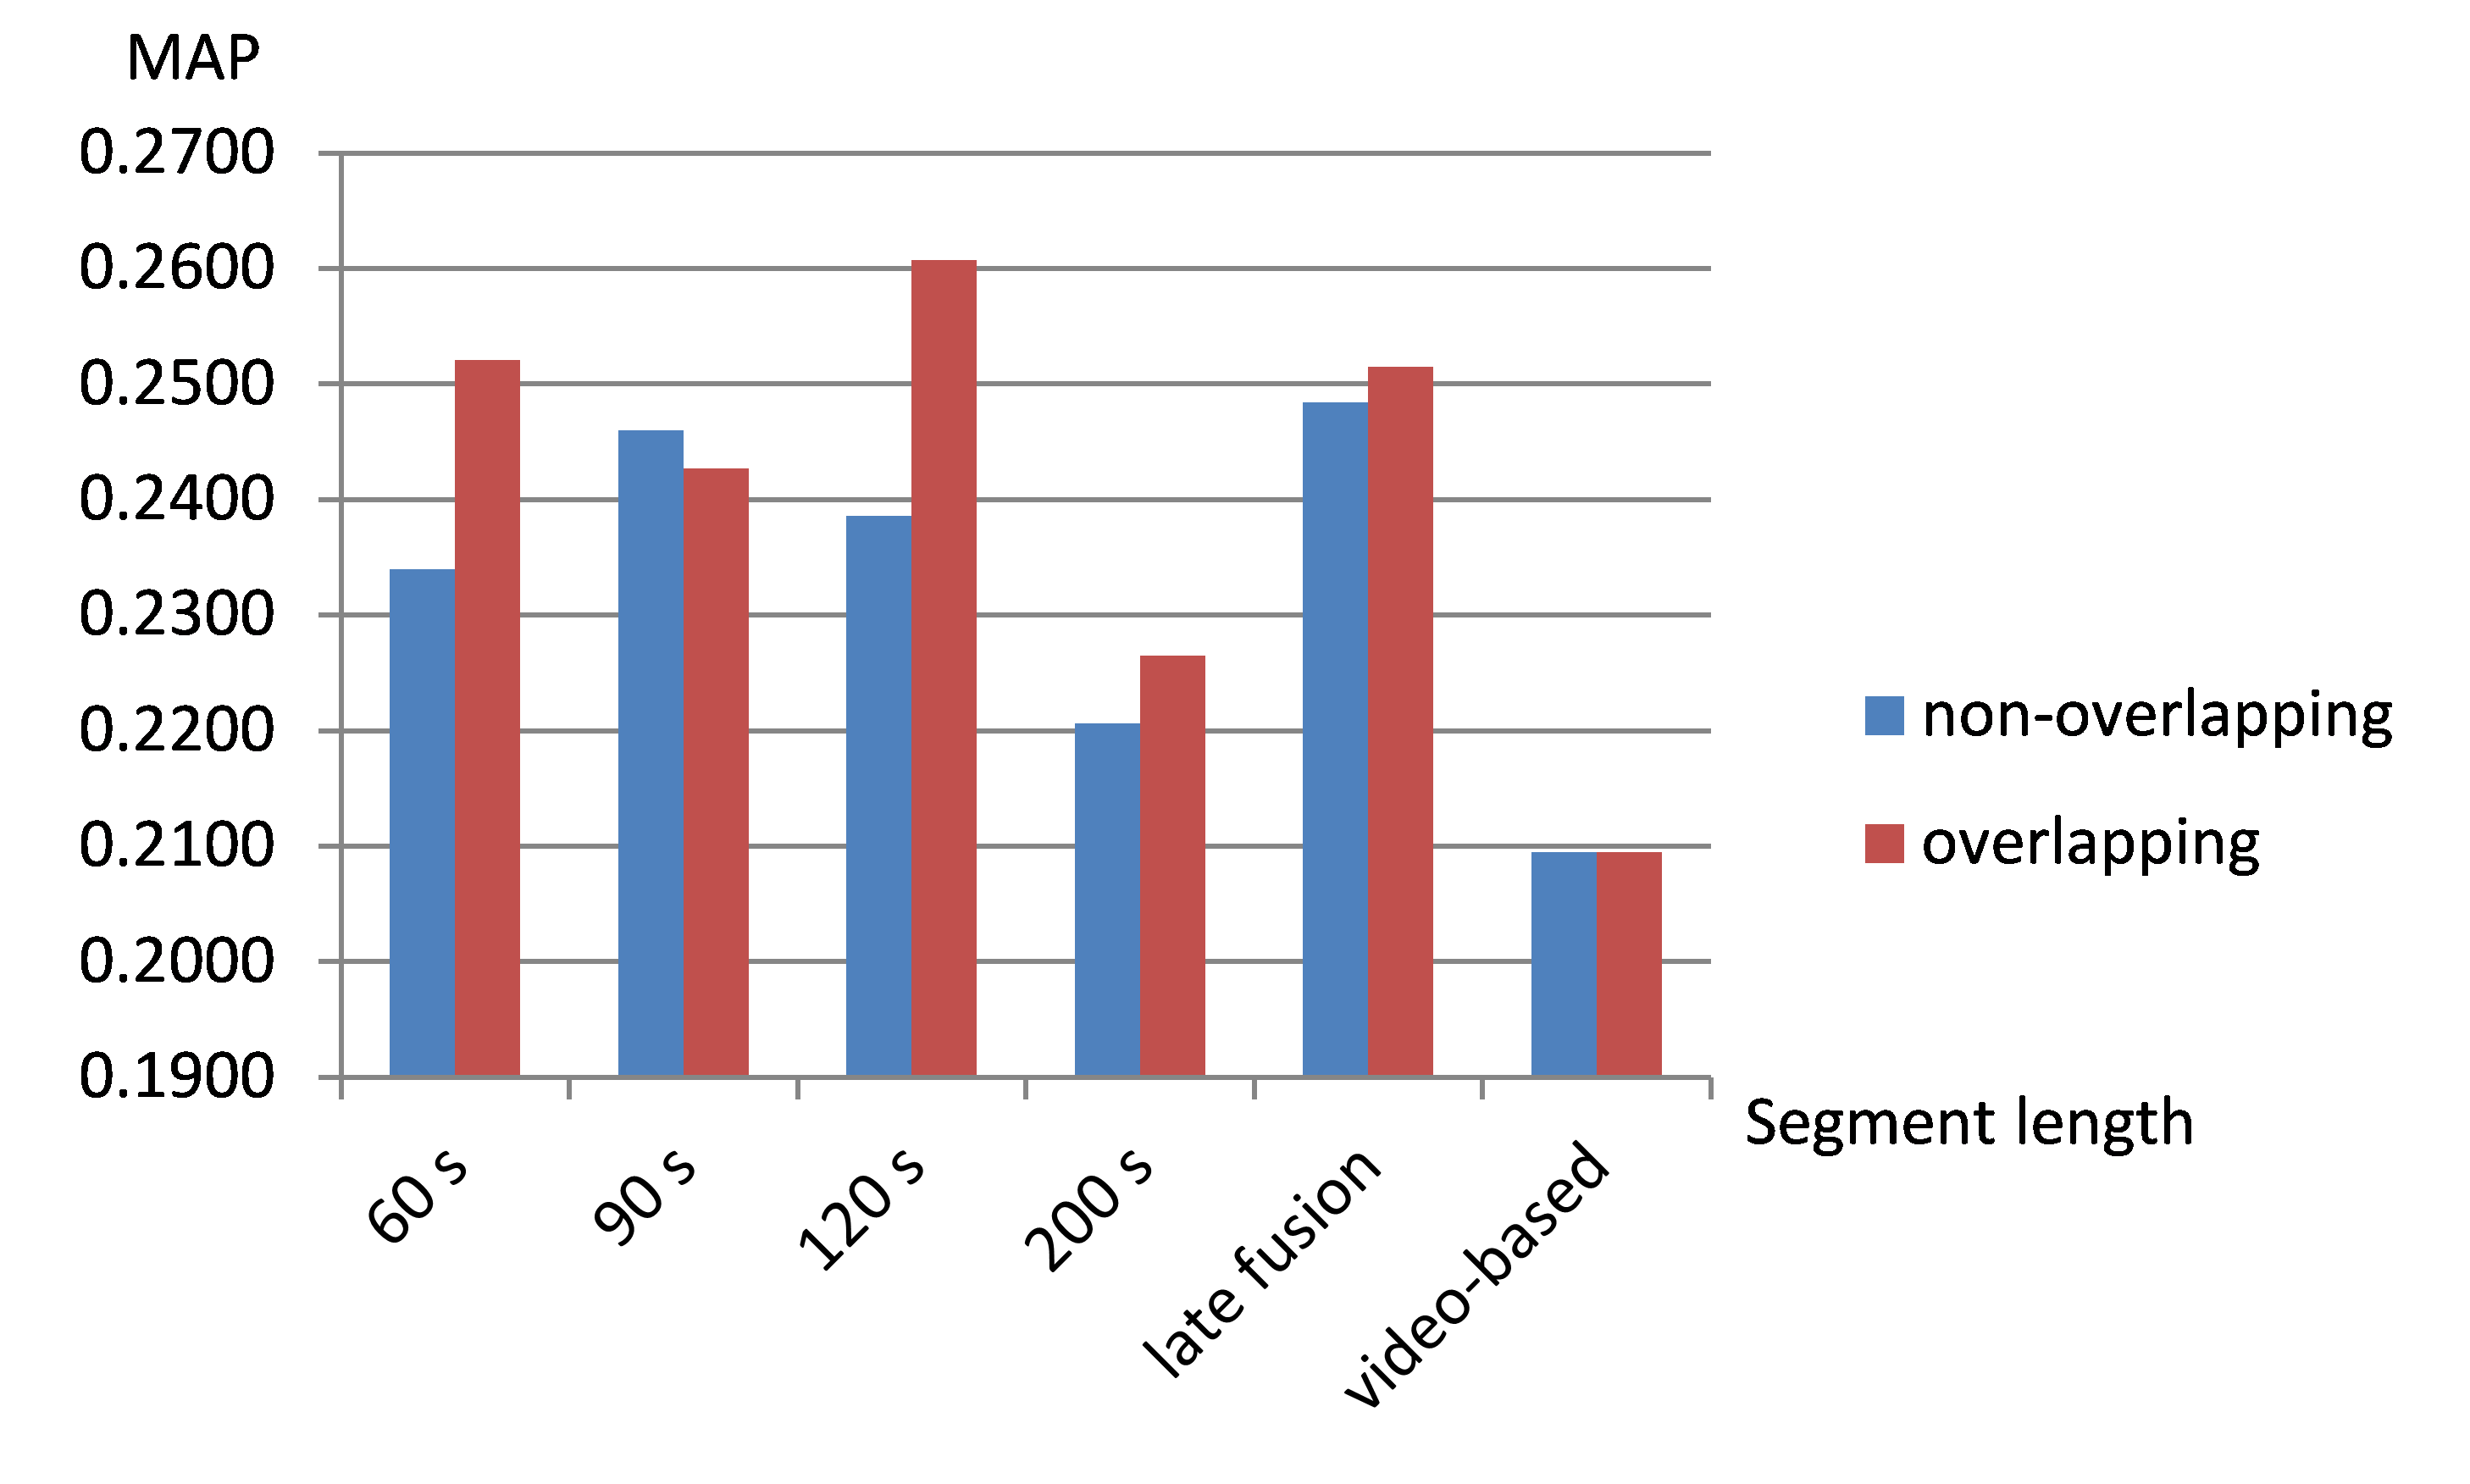
\includegraphics[width=1\textwidth]{images/med11_result.png}}
    (b) On the MED 2011 dataset
  \end{column}
\end{columns}
\bigskip

\begin{itemize}
	\item Segment-based approach significantly outperforms the Video BoW baseline.
	\item In most cases, the overlapping sampling performs the best.
\end{itemize} 

  
\end{frame}

\begin{frame}[t]{Experimental Results: On the MED 2010}
Comparison of different segment-based approaches with the video-based approach on the MED 2010 dataset.
\begin{table}
\renewcommand{\arraystretch}{1.2}
\footnotesize
\centering
% For LaTeX tables use
\begin{tabular}{| p{1.9cm} | p{1.9cm} | p{1.9cm} | p{1.9cm} | p{1.9cm} |}
\toprule
Event/MAP & Best non-overlapping & Best overlapping & SBD segments & Video-based\\
\midrule
Assembling shelter & 0.4511 & 0.4781& 0.4284  & \textbf{0.4911} \\
\midrule
Batting in a run & 0.7852 &\textbf{0.7918}& 0.7866 & 0.7902 \\
\midrule
Making a cake & 0.3636 & \textbf{0.3819} & 0.1918 & 0.2755 \\ 
\midrule
All & 0.5333 & \textbf{0.5506} & 0.4689 & 0.5189 \\
\bottomrule
\end{tabular}
\end{table}

\begin{itemize}
\item Segment-based approach outperforms the video-based approach.
\item Shot boundary detection does not work.
\begin{itemize}
	\item It is difficult to detect shot boundary with high accuracy in real videos.
\end{itemize} 
\end{itemize}

\end{frame}

\begin{frame}[t]{Experimental Results: On the MED 2011}
	\small{Comparison of different segment-based approaches with the video-based approach.}
\begin{table}
	\tiny
	\renewcommand{\arraystretch}{1}
	\label{t_med11_comparison}
	\centering
	\begin{tabular}{|c|c|c|c|c|c|c|c|}
		\hline
		\multirow{3}[4]{*}{Event} & \multicolumn{3}{|c|}{Non-overlapping sampling} & \multicolumn{3}{|c|}{Overlapping sampling} & \multirow{3}[4]{*}{Video-based} \\ 
		\cline{2-7}
		& \begin{tabular}[x]{@{}c@{}}Best\\(at 90 s) \end{tabular}
		& \begin{tabular}[x]{@{}c@{}}Late fusion\\(all lengths) \end{tabular}
		& \begin{tabular}[x]{@{}c@{}}Late fusion\\(60, 90, 120 s) \end{tabular}
		& \begin{tabular}[x]{@{}c@{}}Best\\(at 120 s) \end{tabular}
		& \begin{tabular}[x]{@{}c@{}}Late fusion\\(all lengths) \end{tabular}
		& \begin{tabular}[x]{@{}c@{}}Late fusion\\(60, 90, 120 s) \end{tabular} &  \\ \toprule
		E006  & \multicolumn{1}{|c|}{\textbf{0.1277}} & 0.1217 & 0.1244 & 0.1151 & 0.1086 & \multicolumn{1}{|c|}{0.1083} & 0.0959 \\ \midrule
		
		E007  & \multicolumn{1}{|c|}{0.1521} & 0.1419 & \multicolumn{1}{|c|}{0.1369} & 0.1552 & 0.1610 & \multicolumn{1}{|c|}{\textbf{0.1616}} & 0.1303 \\	\midrule
		E008  & \multicolumn{1}{|c|}{0.4923} & \textbf{0.4975} & \multicolumn{1}{|c|}{0.4973} & 0.4969 & 0.4903 & \multicolumn{1}{|c|}{0.4871} & 0.4766 \\	\midrule
		E009  & \multicolumn{1}{|c|}{0.2072} & 0.2145 & \multicolumn{1}{|c|}{0.2064} & \textbf{0.2160} & 0.1954 & \multicolumn{1}{|c|}{0.1958} & 0.0943 \\	\midrule
		E010  & \multicolumn{1}{|c|}{0.0916} & 0.0771 & \multicolumn{1}{|c|}{0.0753} & 0.1008 & 0.1108 & \multicolumn{1}{|c|}{\textbf{0.1109}} & 0.1020 \\	\midrule
		E011  & \multicolumn{1}{|c|}{0.0698} & 0.0805 & \multicolumn{1}{|c|}{0.0813} & \textbf{0.1591} & 0.0819 & \multicolumn{1}{|c|}{0.0845} & 0.0609 \\	\midrule
		E012  & \multicolumn{1}{|c|}{\textbf{0.3560}} & 0.3309 & \multicolumn{1}{|c|}{0.3277} & 0.3150 & 0.3293 & \multicolumn{1}{|c|}{0.3341} & 0.2858 \\	\midrule
		E013  & \multicolumn{1}{|c|}{0.6030} & 0.6033 & \multicolumn{1}{|c|}{0.6096} & \textbf{0.6188} & 0.5872 & \multicolumn{1}{|c|}{0.5910} & 0.5385 \\	\midrule
		E014  & \multicolumn{1}{|c|}{0.2008} & 0.2585 & \multicolumn{1}{|c|}{0.2579} & \textbf{0.2744} & 0.2706 & \multicolumn{1}{|c|}{0.2694} & 0.2138 \\	\midrule
		E015  & \multicolumn{1}{|c|}{0.1599} & 0.1583 & \multicolumn{1}{|c|}{0.1622} & 0.1562 & 0.1795 & \multicolumn{1}{|c|}{\textbf{0.1795}} & 0.0964 \\ 	\midrule
		All   & \multicolumn{1}{|c|}{0.2460} & 0.2484 & \multicolumn{1}{|c|}{0.2479} & \textbf{0.2607} & 0.2515 & \multicolumn{1}{|c|}{0.2522} & 0.2095 \\	\bottomrule
	\end{tabular}%
\end{table}
\begin{itemize}
	\item Segment-based approach outperforms the video-based approach.
	\item \textbf{Optimal segment length}: approximate the \textbf{mean video length}. 
	\begin{itemize}
		\item Late fusion of several runs around the mean video length.
	\end{itemize}	
\end{itemize}	

\end{frame}

\begin{frame}[t]{Conclusions}

	\begin{enumerate}
		\item \textbf{\small{Segment-based Representation (SB)}}
		\begin{itemize}
			\item Investigate different strategies to \\
			decompose a video into segments.
			\item Study the optimal segment length.
			
		\end{itemize}
			\item \light{Sum-Max Video Aggregation (SM)}
			\item \light{Event-driven Multiple Instance \\
			Learning (EDMIL)}
			
	\end{enumerate}
	
	\begin{tikzpicture}[remember picture,overlay]  
	\node [xshift=-3cm,yshift=-4.5cm] at (current page.north east)
	{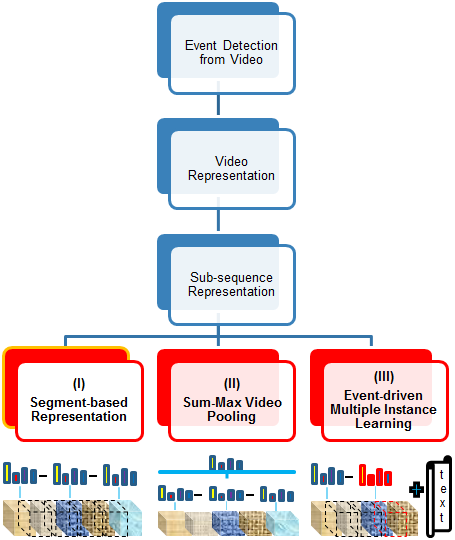
\includegraphics[width=5cm,height=7.5cm]{images/part1/contribution2.png}};
	\end{tikzpicture}
	
\end{frame}

\end{document}

\section{Sum-Max Video Feature Aggregation}


% titlepage-demo.tex
\documentclass{beamer}
\usetheme{Boadilla}
\usepackage{multirow}
\usepackage[absolute,overlay]{textpos} 
\newenvironment{reference}[2]{% 
  \begin{textblock*}{\textwidth}(#1,#2) 
      \footnotesize\it\bgroup\color{red!50!black}}{\egroup\end{textblock*}} 

\begin{document}

%\begin{frame}[t]{Video-based Approach}
%Bag-of-visual-words model: Video level features are aggregated over the entire videos

%\begin{center}
%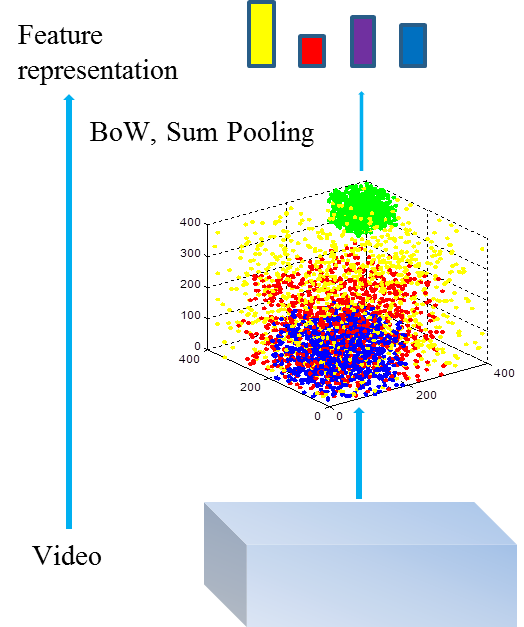
\includegraphics[width=5cm,height=4.5cm]{images/video_based_summax.png}
%\end{center}

%\begin{itemize}
%\item The proposed segment-based approach: increasing the number of segment representation is not scalable. 
%\item \textbf{Specific problem:} How to generate one representation per each video from its segment-level representations?
%\end{itemize}

%\end{frame}

\begin{frame}[t]{How to Detect Event in Video?}
	\begin{itemize}
		\item State-of-the-art systems [Jiang - TRECVID2010], [Natarajan - TRECVID2011] (\textbf{best systems} in TRECVID MED 2010 and 2011)
	\end{itemize}
	
	\begin{center}
		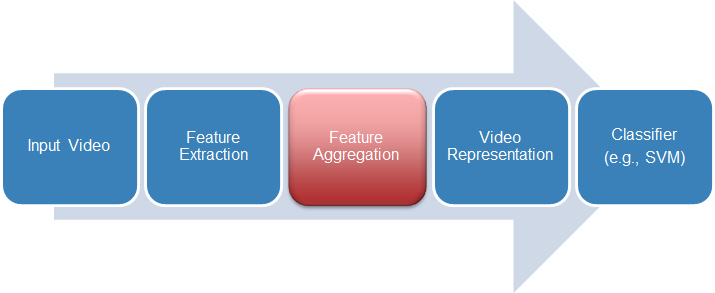
\includegraphics[width=10cm,height=4cm]{images/part3/standardapproach.png}
	\end{center}
	
		\textbf{Problem}: Neutralize the contribution of each part of the whole video. 
		\begin{itemize}
			\item In fact, the clues to determine an event often appear in a small segment.
		\end{itemize}
		
\end{frame}

\begin{frame}[t]{How to Aggregate Feature?}
	\begin{itemize}
		\item \textbf{Sum pooling} strategy [Jiang TRECVID2010], [Natarajan TRECVID2011] (\textbf{best systems} in TRECVID MED 2010 and 2011).
		\begin{itemize}
\item dominant by frequently-occurring descriptors
\item rarely occurring descriptors have less influential
		\end{itemize}	
		
		\item \textbf{Max pooling} strategy [Wang ACCV2012] (often used with sparse coding for image classification [Yang CVPR2009])
				\begin{itemize}
					\item only select the most discriminative information
					\item likely to lost other crucial information
				\end{itemize}	
		\item \textbf{Dynamic pooling} [Li ICCV2013]: dynamically
		determine the pooling operator most suited for each
		sequence using Latent SVM. \\
		$\rightarrow$ very time-consuming!
			
	\end{itemize}
	Problem: How to combine \textbf{Sum pooling} and \textbf{Max pooling} in a efficient way?


\end{frame}

\begin{frame}{Sum-max Video Pooling} 
	\begin{itemize}
\item \textbf{Sum pooling} at lower layer to accumulate sufficient features.
\item \textbf{Max pooling} to retrieve the most relevant features at the high layer.
$\rightarrow$ can discard irrelevant features in the final video representation.
%\bigskip
	\end{itemize}

\begin{columns}
  \begin{column}{0.3\textwidth}
    \centerline{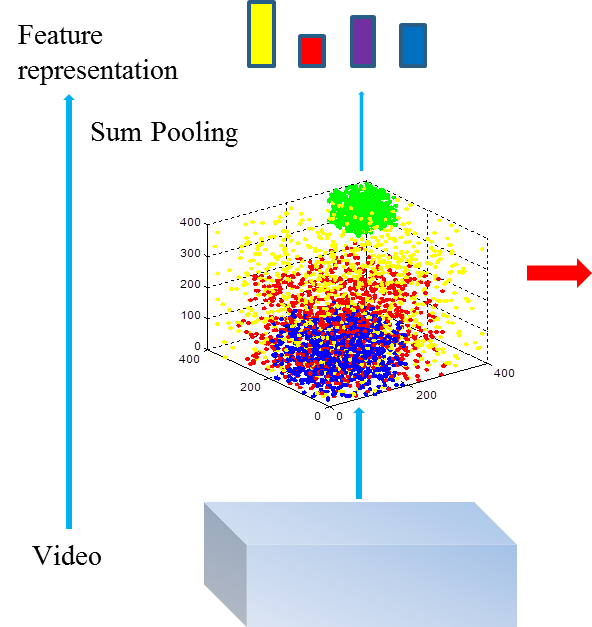
\includegraphics[width=1\textwidth]{images/video_based_summax2.png}}
    (a) The video-based approach
  \end{column}

  \begin{column}{0.7\textwidth}
    \centerline{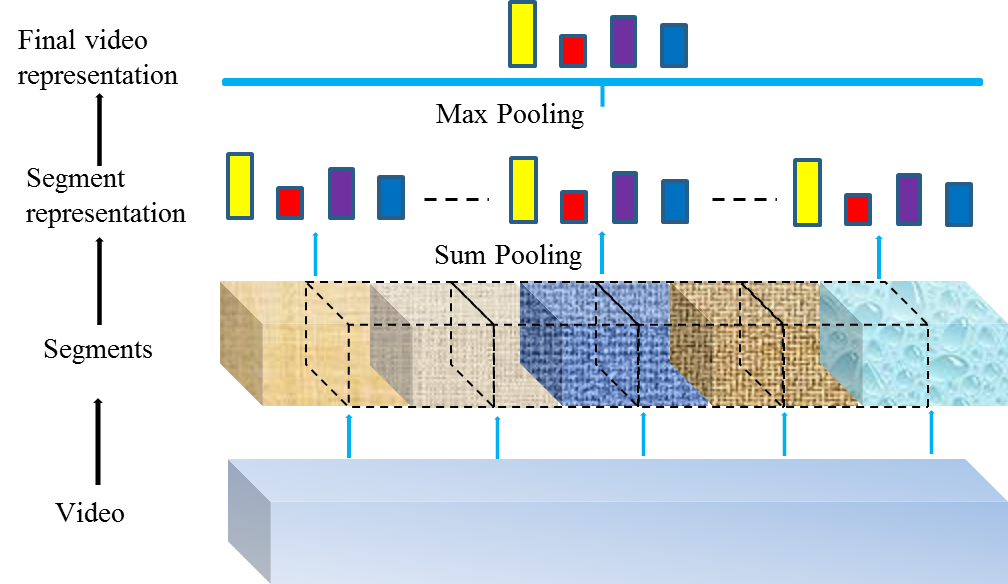
\includegraphics[width=1\textwidth]{images/segment_based_summax.png}}
    (b) \textbf{Our proposed Sum-max Video Pooling}
  \end{column}
\end{columns}
\bigskip
 
  
\end{frame}

\begin{frame}[t]{Sum-max Video Pooling}

\begin{itemize}
	\item Notation:
\begin{itemize}
\item N local descriptors $x_{n} \in R^{D}$, n = 1,...,N and D is the feature dimension
\item K visual words $m_{k} \in R^{D}$, where k = 1,...,K 
\item $M = \{m_{k}\}$ is the set of visual words
\item Coding step: $\phi_{n} = [\Phi_{1n},...,\Phi_{Kn}]$
\item \textit{S} is number of segments
\item $N_{s}$ is the number of local descriptors in segment \textit{s} 
\end{itemize}
\item The sum-max and max-sum video pooling at each visual word can be defined as follows:
\begin{equation}\psi_{k_{\textbf{sum-max}}} = Max_{s \in S}(\sum_{n \in N_{s}}\Phi_{kn})\end{equation}

\begin{equation}\psi_{k_{\textbf{max-sum}}} = \sum_{s \in S}(Max_{n \in N_{s}}\Phi_{kn})\end{equation}
\end{itemize}

\end{frame}

\begin{frame}[t]{Complexity}
	
	\begin{itemize}
		\item Same complexity with the \textbf{sum video pooling}:
		\begin{equation}\psi_{k_{\textbf{sum-max}}} = Max_{s \in S}(\sum_{n \in N_{s}}\Phi_{kn})\end{equation}
		
		\begin{equation}\psi_{k_{\textbf{sum}}} = \sum_{s \in S}(\sum_{n \in N_{s}}\Phi_{kn})\end{equation}
		\item Very efficient
	 	\begin{itemize}
	 		\item Extracting features only once!
	 		\item Aggregating features at different segment lengths efficiently.
		\end{itemize}
	\end{itemize}
		\begin{center}
			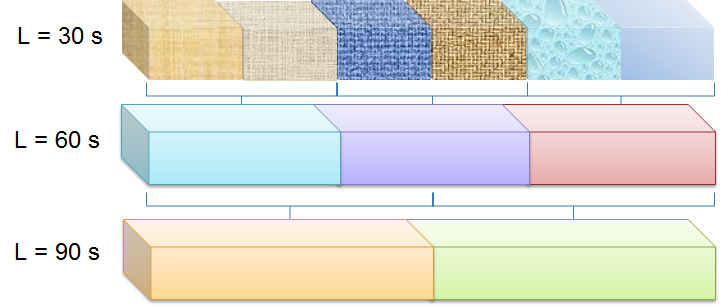
\includegraphics[width=8cm,height=3cm]{images/part3/efficient.png}
			\\	\scriptsize{Features from higher layers can be obtained from lower layers efficiently!}
		\end{center}
\end{frame}

\begin{frame}{Experimental Setup} 	
	\begin{itemize}
		\item Dataset
		
		\begin{table}[h]
			\tiny
			\begin{tabular}{@{}|l|c|c|c|c|c|@{}}
				\toprule
				\multicolumn{1}{|c|}{Dataset} & No. Event & No. Train Videos & No. Test Videos & Total Videos & Total Hours \\ \midrule
				MED2010 & 3 & 1,744 & 1,724 & 3,468 & 110 hours \\ \midrule
				MED2011 & 10 & 1,331 & 31,822 & 33,153 & 1,100 hours \\ \midrule
				\light{MED2012} & \light{25} & \light{3,878} & \light{1,938} & \light{5,816} & \light{250 hours} \\ \bottomrule
			\end{tabular}
		\end{table}
		
		\item Feature: 
			\begin{itemize}
				\item MED10: Dense Trajectories, MBH descriptor [Wang-CVPR2011] 	
				\item MED11: Improved Dense Trajectories, MBH descriptor [Wang-ICCV2013] 	
			\end{itemize}
		\item Feature encoding: Bag-of-words model, 4000 codewords.
		\item Learning: ${\chi}^{2}$ SVM.
	\end{itemize}
	
\end{frame}	

\begin{frame}[t]{Experimental Results: On MED 2010}
\begin{table}
\renewcommand{\arraystretch}{1}
\caption{Performance comparison of different video pooling strategies on the MED 2010 dataset.}
\label{t_med10}
\centering
\begin{tabular}{|c|c|c|c|c|}
\toprule
Event/MAP & \begin{tabular}[x]{@{}c@{}}Max pooling\\(Video-based) \end{tabular} & \begin{tabular}[x]{@{}c@{}}Sum pooling\\(Video-based) \end{tabular} & \begin{tabular}[x]{@{}c@{}}Max-sum\\pooling\\(at 60 s)\end{tabular} & \begin{tabular}[x]{@{}c@{}}Sum-max\\pooling\\(at 60 s)\end{tabular} \\
%\bfseries \begin{tabular}[c]{@{}c@{}} CU\\(SIFT)\end{tabular}&
%\bfseries \begin{tabular}[c]{@{}c@{}}CU (STIP,\\SIFT,\\MFCC)\end{tabular}\\
\midrule
E001&0.4365&0.4468&0.4646&\textbf{0.5072}
\\
\midrule
E002&0.6434&\textbf{0.7988}&0.7103&0.7900
\\
\midrule
E003&\textbf{0.3144}&0.3053&0.2806&0.3100
\\
\midrule
All&0.4648&0.5170&0.4852&\textbf{0.5357}
%&0.512&0.633
\\
\bottomrule
\end{tabular}
\end{table}


\begin{itemize}
\item Pooling over segments is more effective.
\item \textbf{Sum-max video pooling outperforms the traditional video-based sum pooling.}
\end{itemize}
\end{frame}

\begin{frame}[t]{Experimental Results: On MED 2011}
\begin{center}
	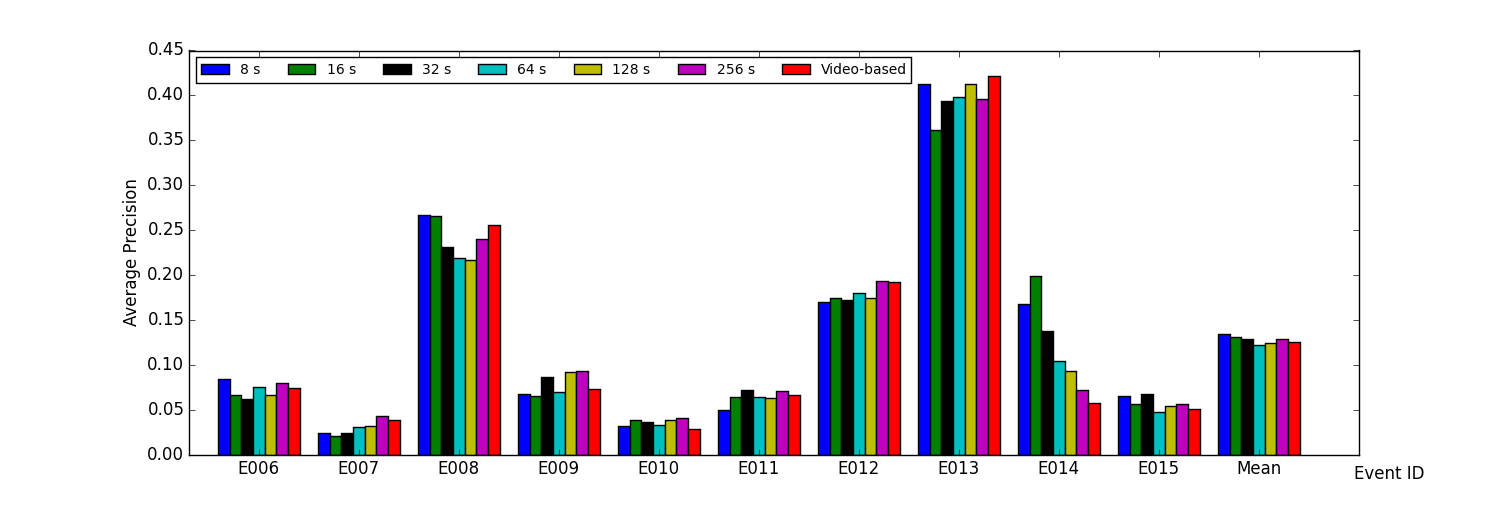
\includegraphics[width=12cm,height=3.5cm]{images/part3/med11_summax_kernel2.png}
	\\	\scriptsize{Results of Sum-max video pooling on the MED 2011 dataset.}

\begin{table}[h]
	\tiny
	\begin{tabular}{@{}|c|c|c|c|c|c|c|c|@{}}
		\toprule
		Method/mAP                                                                   & 8 s       & 16 s      & 32 s   & 64 s   & 128 s  & 256 s  & video-based \\ \midrule
		Sum-Max                                                                      & \textbf{0.1339}    & 0.1311   & 0.1282 & 0.1220 & 0.1242 & 0.1283 & 0.1257      \\ \midrule
		Segment-based                                                                & \multicolumn{2}{c|}{} & 0.1510 & 0.1503 & \textbf{0.1518} & 0.1365 & 0.1257      \\ \bottomrule
%		\begin{tabular}[c]{@{}c@{}}Dynamic Pooling \\ {[}Li-ICCV2013{]}\end{tabular} & \multicolumn{6}{c|}{}                                     & 0.1227      \\ \bottomrule
	\end{tabular}
\end{table}
	
\end{center}
\begin{itemize}
	\item The best performance is at 8 s (\textbf{6}\% improvement!)
	\item Sum-max video pooling performs significantly worse than the segment-based approach!
	\item However, sum-max video pooling is very \textbf{efficient}!
\end{itemize}

\end{frame}

\begin{frame}[t]{Conclusions}
	
	\begin{enumerate}
		\item \light{Segment-based Representation (SB)}
		\item \textbf{Sum-Max Video Aggregation (SM)}
		\begin{itemize}
			\item An efficient method to aggregate\\
			local features into video feature \\
			representation.
		\end{itemize}
		\item \light{Event-driven Multiple Instance \\
			Learning (EDMIL)}
	\end{enumerate}
	
	
	\begin{tikzpicture}[remember picture,overlay]  
	\node [xshift=-3cm,yshift=-4.5cm] at (current page.north east)
	{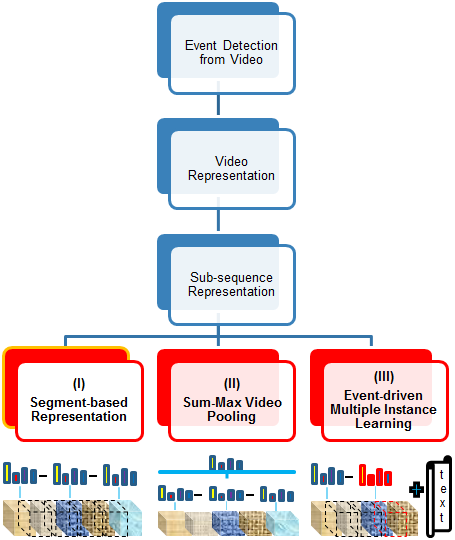
\includegraphics[width=5cm,height=7.5cm]{images/part1/contribution2.png}};
	\end{tikzpicture}
	
\end{frame}



\end{document}

\section{Event-driven Multiple Instance Learning}


% titlepage-demo.tex
\documentclass{beamer}
\usetheme{Boadilla}
\usepackage{multirow}
\usepackage[absolute,overlay]{textpos} 
\newenvironment{reference}[2]{% 
  \begin{textblock*}{\textwidth}(#1,#2) 
      \footnotesize\it\bgroup\color{red!50!black}}{\egroup\end{textblock*}} 

\begin{document}

\begin{frame}{Motivation - Human Way to Detect Event} 
	\begin{center}
		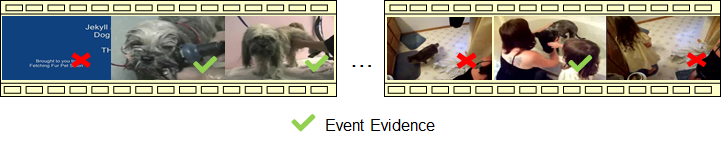
\includegraphics[width=11cm,height=3cm]{images/part4/minimalevidence.png}
	\end{center}
	\begin{itemize}
		\item Human only needs to see some evidences.
		\item Leveraging on positive and negative visual cues selected by humans significantly improves the performance.
	\end{itemize}
 \begin{reference}{4mm}{85mm}
 	Bhattacharya, S., Yu, F. X., Chang, S. F. Minimally needed evidence for complex event recognition in unconstrained videos. In ICMR. ACM, 2014.
 \end{reference}  
\end{frame}

\begin{frame}{Motivation - Not Easy for Computer} 
	\begin{center}
		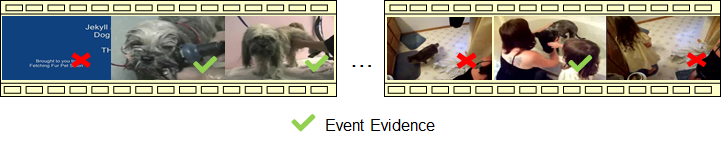
\includegraphics[width=11cm,height=3cm]{images/part4/minimalevidence.png}
	\end{center}
	
	\begin{itemize}
		\item How to detect which segments of the video that have the most contributions? 	
		\item How to leverage these ``\textit{key evidences}'' for event detection?
	\end{itemize}	
	$\rightarrow$ Answering these two questions can help understand why an event is detected.	
\end{frame}

\begin{frame}{Weakly Supervised Learning Problem} 	
	\textbf{\textit{Problem}}: Event labels are only given at video level!
	
	\begin{center}
		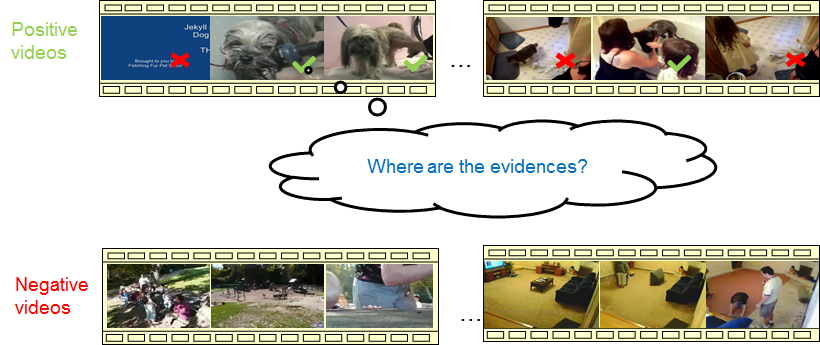
\includegraphics[width=11cm,height=4cm]{images/part4/supervidedlearning.png}
	\end{center}
	
	
	\textbf{Related work} 
	\begin{itemize}	
		\item Latent SVM [Tang-CVPR2012], [Li-ICCV2013]
		\item \textbf{Multiple Instance Learning} [Zhang-ICML2002], [Lai-CVPR2014] 
			\begin{itemize}	
\item Mathematically equivalent to Latent SVM! 
\item MIL can be applied directly to learn labels at segment level: \\
video $\rightarrow$ ``bag'', segment $\rightarrow$ ``instance''.
			\end{itemize}	
	\end{itemize}	

\end{frame}	

\begin{frame}{Multiple Instance Learning - miSVM} 	
	Two key assumptions of MIL:
	\begin{itemize}	
		\item A positive bag has \textbf{at least} one positive instance.
		\item The instances in a negative bag are \textbf{all} negatives.
	\end{itemize}	
	\begin{center}
		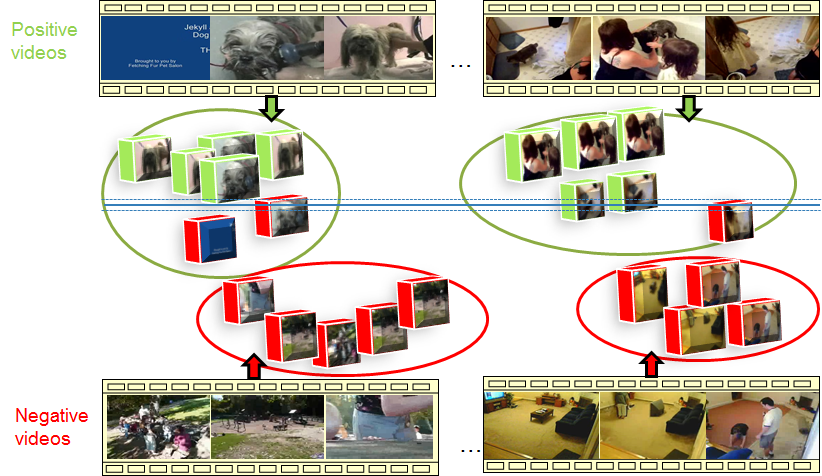
\includegraphics[width=11cm,height=6cm]{images/part4/miSVM.png}
		\\
		\scriptsize{miSVM: instance-based classifier}
	\end{center}
	
\end{frame}	

\begin{frame}{Multiple Instance Learning - MISVM} 	

	\begin{center}
		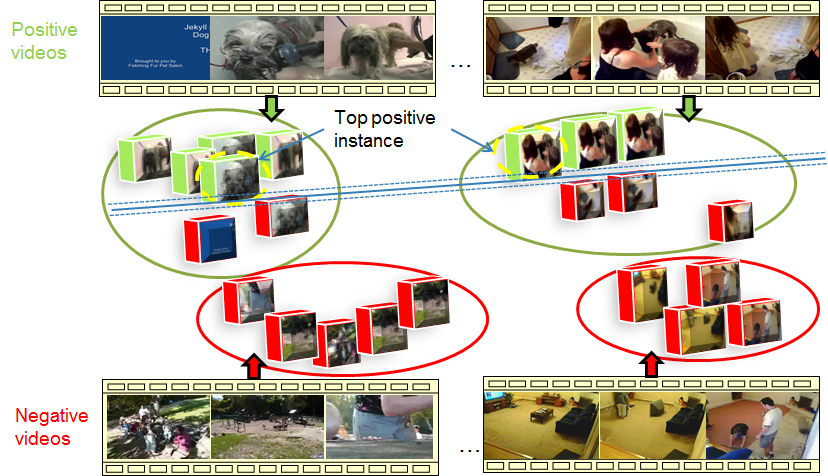
\includegraphics[width=11cm,height=6cm]{images/part4/MI-SVM.png}
		\\
		\scriptsize{MISVM: bag-based classifier}
	\end{center}
\textbf{Limitations}: MIL assumptions may not be valid for videos, esp. \textbf{complex} videos.
\end{frame}	

\begin{frame}{Proportional SVM [Lai-CVPR2014]} 	
	Two new assumptions of p-SVM:
	\begin{itemize}	
		\item Positive videos should have \textbf{high proportion} of positive instances.
		\item Negative videos could have \textbf{some} positive instances.
	\end{itemize}	
	
	\begin{center}
		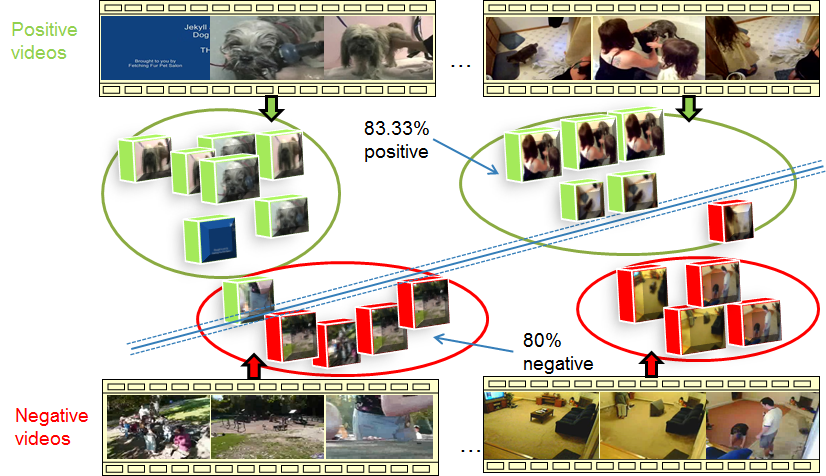
\includegraphics[width=11cm,height=6cm]{images/part4/pSVM.png}
	\end{center}
	
\end{frame}	

\begin{frame}{Our Proposed Method} 	
	
\begin{itemize}	
	\item \textbf{Limitation} of previous work: weakly supervised learning problem
	\begin{itemize}	
		\item Instance labels are solely classified based on its represented feature in a large margin framework.
		\item The importance of each instance is not considered.
	\end{itemize}	
	
	\item What if we know information about the instance labels?
		\begin{itemize}	
			\item E.g., the relatedness of each instance to the event of interest.
		\end{itemize}	
		\begin{center}
			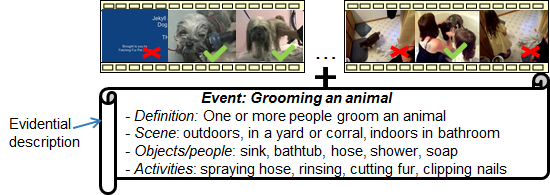
\includegraphics[width=9cm,height=4cm]{images/part4/eventkit.png}
		\end{center}
	\item \textbf{Our proposed method}: A ``stronger'' supervised learning problem
		\begin{itemize}	
			\item Event-driven Multiple Instance Learning (EDMIL) to utilize the \textit{evidential description} for event detection.
		\end{itemize}	

\end{itemize}	
	
\end{frame}	

\begin{frame}{Instance-Event Similarity} 	
	\begin{itemize}	
		\item Adopt a \textbf{concept expansion} strategy [Wang ICMR2014]
				\begin{itemize}	
					\item Apply at instance level
				\end{itemize}	
	\item consists of 4 steps:
	
		\begin{itemize}
			\item Concept detection.
			\item Event representation (text-based).
			\item Concept-event similarity.
			\item Instance-event similarity.
		\end{itemize}
		
	\end{itemize}		
	\begin{center}
		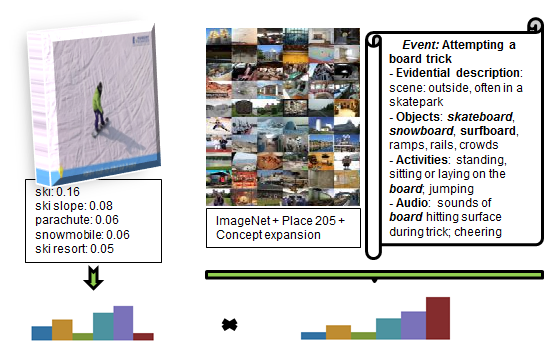
\includegraphics[width=9cm,height=4.7cm]{images/part4/similarity.png}
	\end{center}

\end{frame}	

\begin{frame}{Instance-Event Similarity (cont'd)} 	

% Please add the following required packages to your document preamble:
% \usepackage{booktabs}
\begin{table}[h]
	\scriptsize
		\caption{Top five concepts discovered by our system for the first 10 events in the MED 2012 dataset.}
		\renewcommand{\arraystretch}{0.8}
	\begin{tabular}{@{}ll@{}}
		\toprule
		\multicolumn{1}{c}{\textbf{Event name}}                & \multicolumn{1}{c}{\textbf{Top five importance concepts discovered by our system}}                                                  \\ \midrule
		\multicolumn{1}{|l|}{Attempting a board trick}         & \multicolumn{1}{l|}{Ski, slide rule, ski resort, ski mask, ice skating rink}                                                        \\ \midrule
		\multicolumn{1}{|l|}{Feeding an animal}                & \multicolumn{1}{l|}{Meat loaf, white shark, food court, pop bottle, cleaver}                                                        \\ \midrule
		\multicolumn{1}{|l|}{Landing a fish}                   & \multicolumn{1}{l|}{Anemone fish, pole, raft, sturgeon, boat deck}                                                                  \\ \midrule
		\multicolumn{1}{|l|}{Wedding ceremony}                 & \multicolumn{1}{l|}{Groom, bridegroom, banquet hall, gown, altar}                                                                   \\ \midrule
		\multicolumn{1}{|l|}{Working on a woodworking project} & \multicolumn{1}{l|}{\begin{tabular}[c]{@{}l@{}}Jigsaw puzzle, bamboo forest, carpenter's kit, thatch,\\  wooden spoon\end{tabular}} \\ \midrule
		\multicolumn{1}{|l|}{Birthday party}                   & \multicolumn{1}{l|}{Table lamp, lampshade, torch, candle, custard apple}                                                            \\ \midrule
		\multicolumn{1}{|l|}{Changing a vehicle tire}          & \multicolumn{1}{l|}{\begin{tabular}[c]{@{}l@{}}Recreational vehicle, car wheel, amphibian, scooter,\\  sports car\end{tabular}}     \\ \midrule
		\multicolumn{1}{|l|}{Flash mob gathering}              & \multicolumn{1}{l|}{Monitor, chime, bell, whistle, ballroom}                                                                        \\ \midrule
		\multicolumn{1}{|l|}{Getting a vehicle unstuck}        & \multicolumn{1}{l|}{\begin{tabular}[c]{@{}l@{}}Recreational vehicle, amphibian, tank, car wheel,\\  motor scooter\end{tabular}}     \\ \midrule
		\multicolumn{1}{|l|}{Grooming an animal}               & \multicolumn{1}{l|}{Nail, bathtub, shower, fur coat, washbashin}                                                                    \\ \bottomrule
	\end{tabular}
\end{table}
	
\end{frame}	

\begin{frame}{Event-driven Multiple Instance Learning} 	
	
	\begin{itemize}	
		\item $V$: number of training videos
		\item $I_{v}$: number of instances in video $v$
		\item $S_{iv}^{e}$: similarity between instance $iv$ and event $e$ 
		\item R: number of level of relatedness from an instance to an event
	\end{itemize}
We define two predict functions for positive and negative instances at level $r$ as follows. \\
	\begin{center}
$
P_{pos}(S_{iv}^{e},r) = 
\begin{cases}
1,& \text{if } Rank(S_{iv}^{e}) \leq r \\
-1,              & \text{otherwise}
\end{cases}
$

$
P_{neg}(S_{iv}^{e},r) = 
\begin{cases}
-1,& \text{if } Rank(S_{iv}^{e}) \leq r \\
1,              & \text{otherwise}
\end{cases}
$
\end{center}

$Rank(.)$ is the function to quantize a similarity into a related level.
\textbf{Intuition}: we can select the top positive and negative instances at each level of relatedness $r$.
\end{frame}	



\begin{frame}{Event-driven Multiple Instance Learning} 	
		\begin{itemize}	
			\item Objective function
		\end{itemize}	
	\begin{center}
		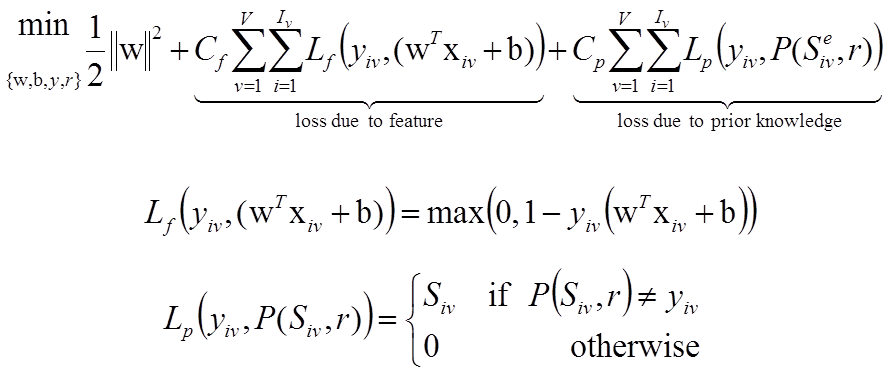
\includegraphics[width=10cm,height=4.5cm]{images/part4/formalization.png}
		\\
		$C_{f}$, $C_{p}$: cost parameters to control the influence of each loss function.\\
				
	\end{center}
\begin{itemize}	
	\item Mixed-integer programming problem $\rightarrow$ \textbf{non-convex optimization}!
\end{itemize}	
	
\end{frame}	

\begin{frame}{Optimization Procedure} 	

		\textbf{Alternating optimization strategy} to search for a suboptimal solution:

\begin{enumerate}
	\item Fix instance labels $y_{iv}$ and solve for \textbf{w} and \textit{b} $\rightarrow$ classic SVM problem:
	
		\begin{center}
	\small{$\min\limits_{\textbf{w},b}$ $\frac{1}{2} \left \| \textbf{w} \right \|^{2} + C_{f} \sum_{v=1}^{V}\sum_{i=1}^{I_{v}}L_{f}\left ( y_{iv}, \textbf{w}^{T}\textbf{x}_{iv}+b \right )$}
		\end{center}
	
	\item Fix \textbf{w} and \textit{b}, solve for $r$ and update $y_{iv}$:
	
		\begin{center}
	\small{$\min\limits_{y,r} C_{f} \sum_{v=1}^{V}\sum_{i=1}^{I_{v}}L_{f}\left ( y_{iv}, \textbf{w}^{T}\textbf{x}_{iv}+b \right )
	+ C_{p} \sum_{v=1}^{V}\sum_{i=1}^{I_{v}}L_{p}\left ( y_{iv}, P(S_{iv}^{e},r) \right )$}
		\end{center}
		
		Solved by using a \textbf{greedy strategy}: 
		\begin{itemize}
			\item Iterate through all level of relatedness to search for the optimal $r$.
			\item Update instance labels $y_{iv}$ using the proposed predict functions.
		\end{itemize}
		\textbf{Intuition}: the most positive and negative instances will be selected first $\rightarrow$ higher possibility to correct mismatched labels.
\end{enumerate}
	
	
\end{frame}	

\begin{frame}{Experimental Setup} 	
	\begin{itemize}
		\item Dataset

\begin{table}[h]
	\tiny
	\begin{tabular}{@{}|l|c|c|c|c|c|@{}}
		\toprule
		\multicolumn{1}{|c|}{Dataset} & No. Event & No. Train Videos & No. Test Videos & Total Videos & Total Hours \\ \midrule
		\light{MED2010} & \light{3} & \light{1,744} & \light{1,724} & \light{3,468} & \light{110 hours} \\ \midrule
		MED2011 & 10 & 1,331 & 31,822 & 33,153 & 1,100 hours \\ \midrule
		MED2012 & 25 & 3,878 & 1,938 & 5,816 & 250 hours \\ \bottomrule
	\end{tabular}
\end{table}

\item Segment length: 8 seconds [Vahdat ICCV2013]
\item Feature: Improved Dense Trajectories, MBH descriptor [Wang ICCV2013] 
\item Feature encoding: Bag-of-words model, 4000 codewords.
\item Learning: EDMIL (with linear SVM).
\item Testing: Video-level score is obtained by averaging over all instance scores.
	\end{itemize}
		
\end{frame}	


\begin{frame}{Optimal Number of Related Levels} 	
	Select R in the range from 1 to 10 and report the best result.
		\begin{center}
			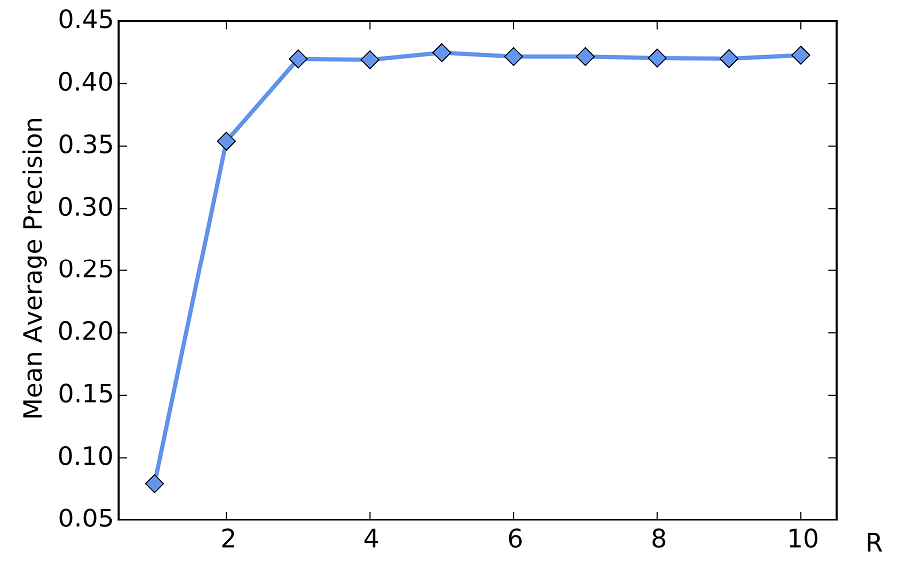
\includegraphics[width=7cm,height=4.5cm]{images/part4/optimalR.png}
		\end{center}

	\begin{itemize}
		\item Small	values of R tend to get low performances $\rightarrow$ the prediction of prior knowledge is not always good, and learning jointly with instance features is necessary.
		\item The performance becomes saturated when R $>$ 5 $\rightarrow$ we fix the value of R to 5 for further experiments.
	\end{itemize}
		
\end{frame}	

\begin{frame}{Results on MED2012} 	
	\begin{center}
		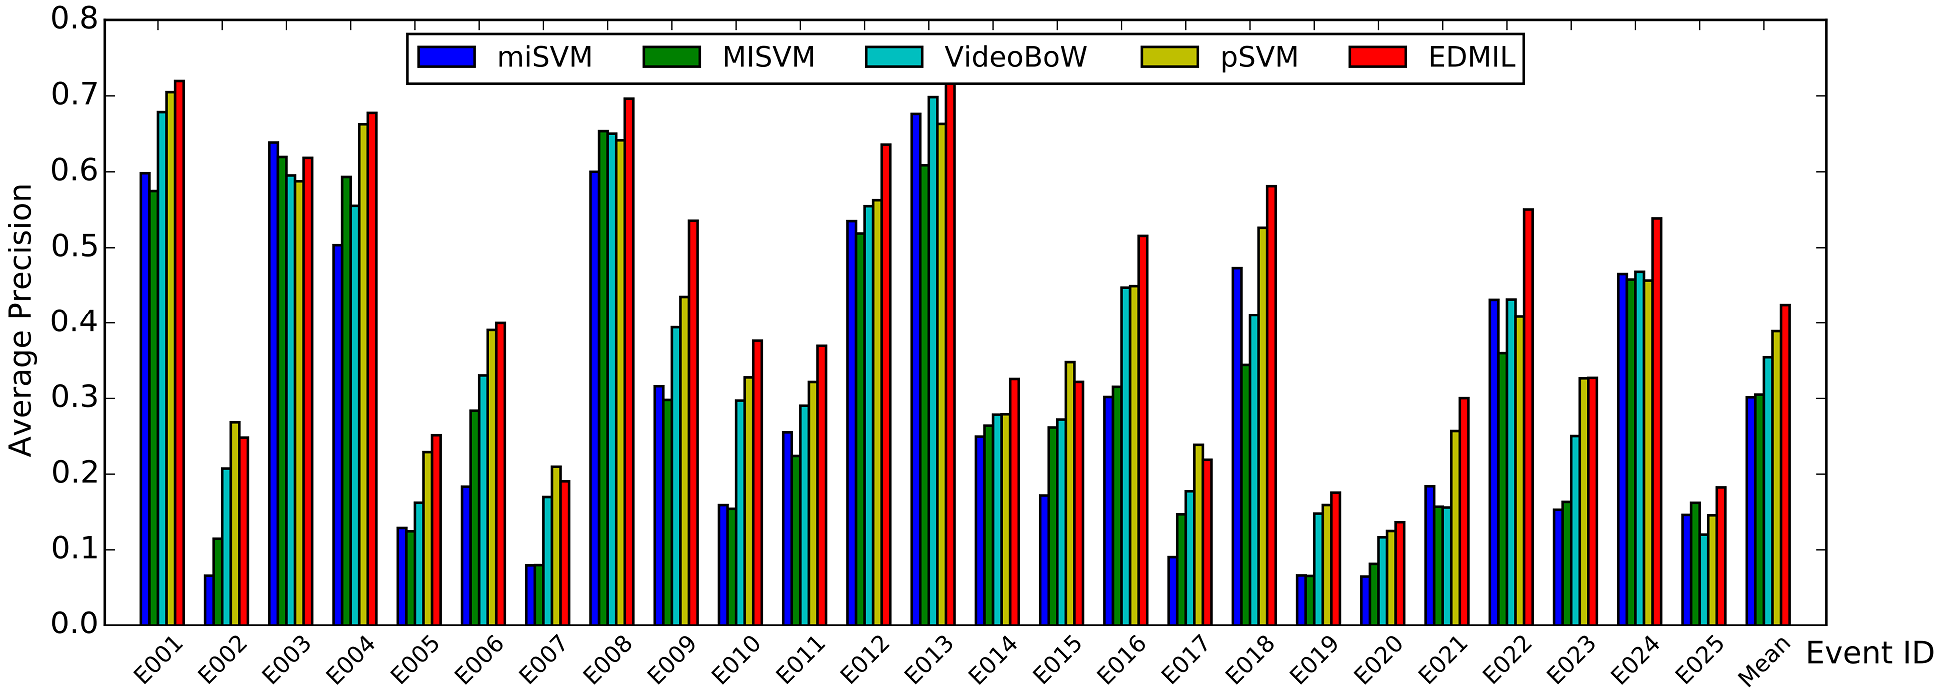
\includegraphics[width=12cm,height=5cm]{images/part4/med12.png}
		\\
		\tiny{The mean APs are 0.3015 (miSVM), 0.3051 (MISVM), 0.3544 (VideoBOW), 0.3890 (pSVM) and \textbf{0.4246} (\textbf{Ours}).}
	\end{center}
	
	\begin{itemize}
		\item Our method significantly outperforms other baselines.
		\item For the best baseline (pSVM), our method relatively outperforms by 9\%. 	
	\end{itemize}
	
\end{frame}	

\begin{frame}{Results on MED2011} 	
	\begin{center}
		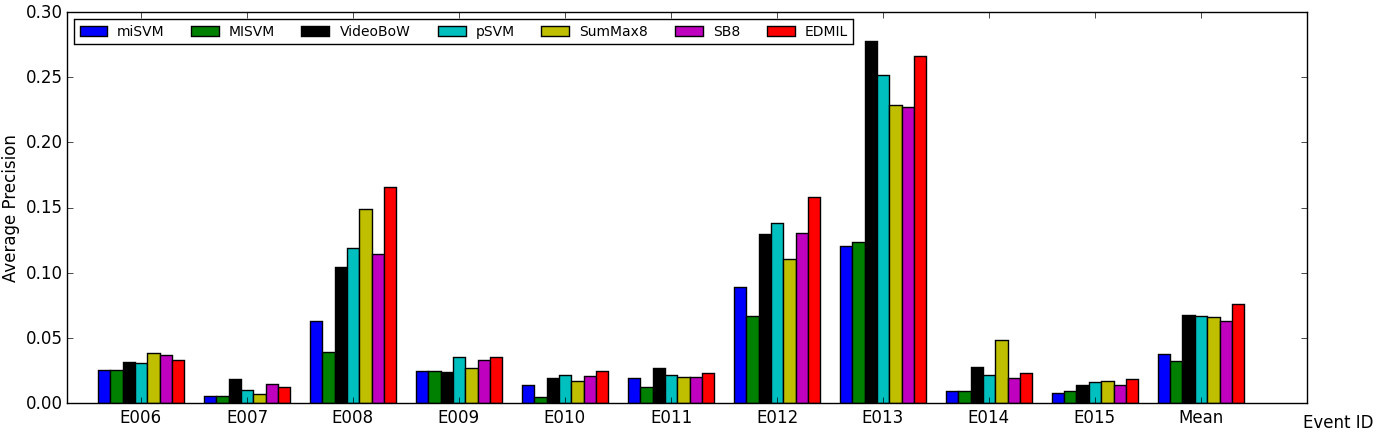
\includegraphics[width=12cm,height=4.5cm]{images/part4/sum_med11_2.png}
		\\
		\tiny{MAP: 0.0378 (miSVM), 0.0322 (MISVM), 0.0674 (VideoBOW), 0.0666 (pSVM), 0.0663 (SM8), 0.0630 (SB8), \textbf{0.0761} (\textbf{Ours}).}
	\end{center}
	
	\begin{itemize}
		\item Our method still performs well (\textbf{13\%} improvement over the VideoBOW baseline) while pSVM does not.
		%\item miSVM performs better than MISVM $\rightarrow$ instance-based learning is more effective.
	\end{itemize}
(At the testing step: Video-level score is obtained by \textbf{averaging} its instance scores.)	
\end{frame}	

\begin{frame}{Results on MED2011} 	
At the testing step: Video-level score is obtained by choosing the \textbf{max} instance score.	
	\begin{center}
		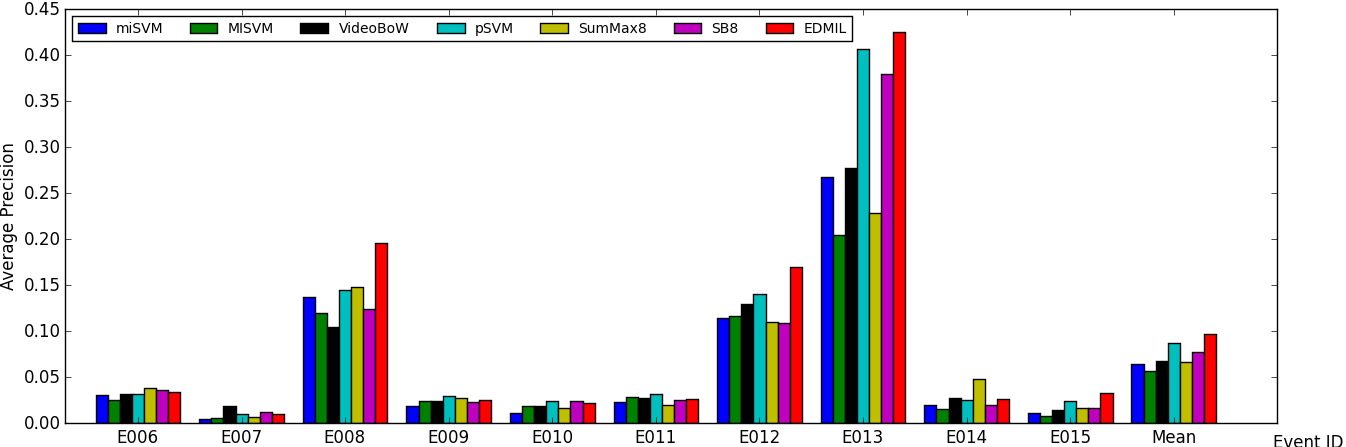
\includegraphics[width=12cm,height=4.5cm]{images/part4/max_med11_2.png}
		\\
		\tiny{MAP: 0.0640 (miSVM), 0.0564 (MISVM), 0.0674 (VideoBOW), 0.0870 (pSVM), 0.0663 (SM8), 0.0770 (SB8), \textbf{0.0968} (\textbf{Ours}).}
	\end{center}
	
	\begin{itemize}
		\item All methods perform better with this strategy.
		\item Our method relatively outperforms VideoBOW by \textbf{44}\%, and pSVM by \textbf{11}\%. 	
	\end{itemize}
	
\end{frame}	

\begin{frame}{How to Leverage ``\textit{Key Evidences}'' for Event Detection?} 	
	$\rightarrow$ At the testing step, video-level score should be obtained by choosing the \textbf{max} instance score.	
	\begin{center}
		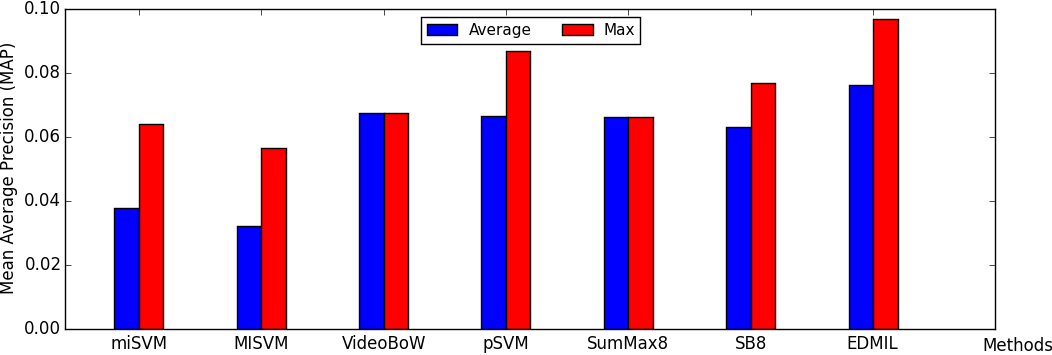
\includegraphics[width=12cm,height=4.5cm]{images/part4/summaxgain.png}
		\\
		Performance gain when choosing the video score as its \textbf{max} instance scores instead of its \textbf{average} instance scores.
	\end{center}
	
\end{frame}	

%\begin{frame}{Top Positive Instances for Event ``Birthday Party''} 	
%
%	\begin{center}
%		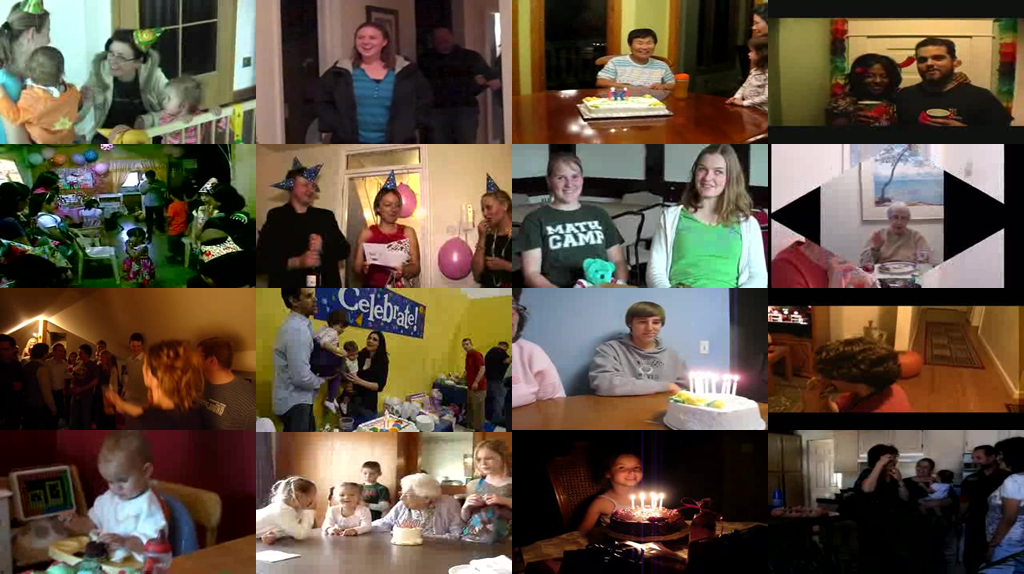
\includegraphics[width=12cm,height=7cm]{images/part4/birthdayparty.png}
%	\end{center}
%	
%\end{frame}	
%
%\begin{frame}{Top Negative Instances for Event ``Birthday party''} 	
%	
%	\begin{center}
%		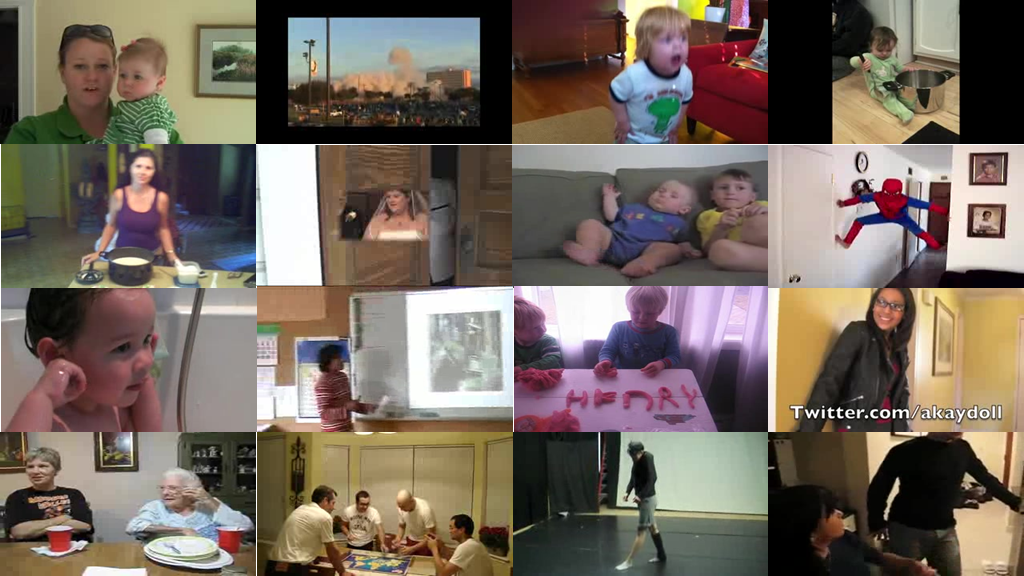
\includegraphics[width=12cm,height=7cm]{images/part4/birthdayparty_neg.png}
%	\end{center}
%	
%\end{frame}	
%
%\begin{frame}{Top Positive Instances for Event ``Flash mob gathering''} 	
%	
%	\begin{center}
%		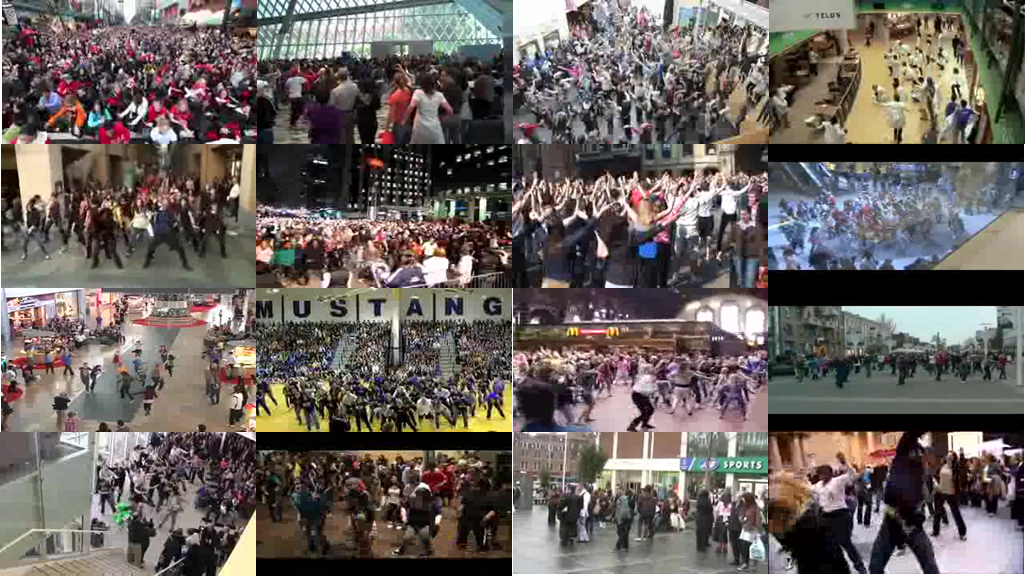
\includegraphics[width=12cm,height=7cm]{images/part4/flashmob.png}
%	\end{center}
%	
%\end{frame}	
%
%\begin{frame}{Top Negative Instances for Event ``Flash mob gathering''} 	
%	
%	\begin{center}
%		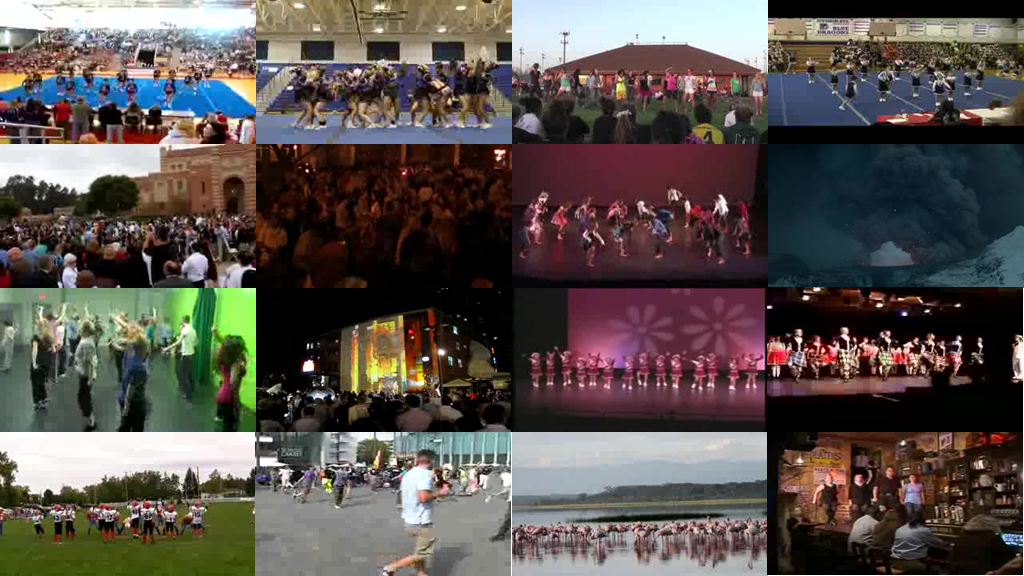
\includegraphics[width=12cm,height=7cm]{images/part4/flashmob_neg.png}
%	\end{center}
	
%\end{frame}	

%\begin{frame}{Top Positive Instances for Event ``Parade''} 	
	
%	\begin{center}
%		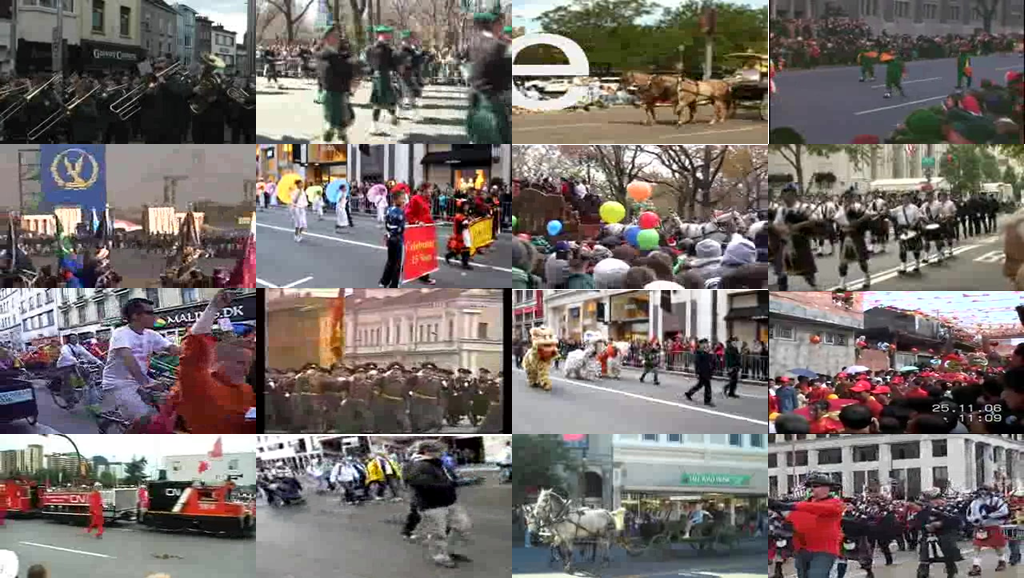
\includegraphics[width=12cm,height=7cm]{images/part4/parade.png}
%	\end{center}
	
%\end{frame}	

%\begin{frame}{Top Negative Instances for Event ``Parade''} 	
	
%	\begin{center}
%		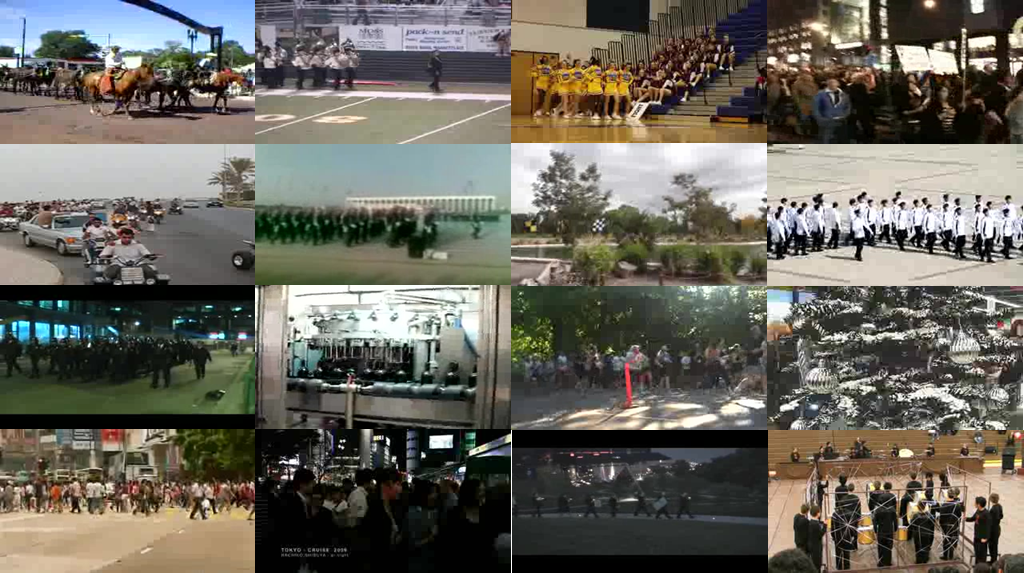
\includegraphics[width=12cm,height=7cm]{images/part4/parade_neg.png}
%	\end{center}
	
%\end{frame}	

\begin{frame}{Top Positive Instances for Event ``Parkour''} 	
\small{\textit{Parkour}: A person travels by foot from one point to another while performing various gymnastic maneuvers.}	
	\begin{center}
		\includegraphics[width=12cm,height=7cm]{images/part4/parkour.png}
	\end{center}
	
\end{frame}	

\begin{frame}{Top Negative Instances for Event ``Parkour''} 	
\small{\textit{Parkour}: A person travels by foot from one point to another while performing various gymnastic maneuvers.}	
	\begin{center}
		\includegraphics[width=12cm,height=7cm]{images/part4/parkour_neg.png}
	\end{center}
	
\end{frame}	



\begin{frame}[t]{Conclusions}
	
	\begin{enumerate}
		\item \light{Segment-based Representation (SB)}
		\item \light{Sum-Max Video Aggregation (SM)}
		\item \textbf{Event-driven Multiple Instance \\
		Learning (EDMIL)}
		\begin{itemize}
			\item A method to leverage the event\\
			description to learn key evidences \\
			for complex event detection.
		\end{itemize}
	\end{enumerate}
	
	\begin{tikzpicture}[remember picture,overlay]  
	\node [xshift=-3cm,yshift=-4.5cm] at (current page.north east)
	{\includegraphics[width=5cm,height=7.5cm]{images/part1/contribution2.png}};
	\end{tikzpicture}
	
\end{frame}


\end{document}

\section{Summary}

% titlepage-demo.tex
\documentclass{beamer}
\usetheme{Boadilla}
\usepackage{multirow}
\usepackage[absolute,overlay]{textpos} 
\newenvironment{reference}[2]{% 
  \begin{textblock*}{\textwidth}(#1,#2) 
      \footnotesize\it\bgroup\color{red!50!black}}{\egroup\end{textblock*}} 



\begin{document}
	

\begin{frame}[t]{Summary}
	
	\begin{enumerate}
		\item \small{Segment-based Representation (SB)}
		\begin{itemize}
			\item \small{Investigate different strategies to \\
				decompose a video into segments; \\
				study the optimal segment length.}
			%\item Outcome: PCM 2012, \textbf{JSPS \\2014} (journal).
			\item \textit{Challenges: uncontrolled capturing, 
				\\large content variation.}
		\end{itemize}
		\item Sum-Max Video Aggregation (SM)
		\begin{itemize}
			\item An efficient method to aggregate\\
			local features into video feature \\
			representation.
			%\item Outcome: ICIP 2014.
			\item \textit{Challenges: uncontrolled capturing,
				\\ large scale dataset.}
		\end{itemize}
		\item Event-driven Multiple Instance \\
		Learning (EDMIL)
		\begin{itemize}
			\item A method to leverage the event\\
			description to learn key evidences \\
			for complex event detection.
			%\item Outcome: ACM MM 2015.
			\item \textit{Challenges: uncontrolled capturing, 
				\\large content variation.}
		\end{itemize}
	\end{enumerate}
	
	\begin{tikzpicture}[remember picture,overlay]  
	\node [xshift=-3cm,yshift=-4.5cm] at (current page.north east)
	{\includegraphics[width=5cm,height=7.5cm]{images/part1/contribution2.png}};
	\end{tikzpicture}
	
\end{frame}


\begin{frame}[t]{Summary (cont'd)}
	
	
	\bigskip
	
	\begin{columns}
		\begin{column}{0.5\textwidth}
			\centerline{\includegraphics[width=1\textwidth]{images/summary3.png}}
			\small{Our methods (SB, SM and EDMIL) improve the baseline VideoBOW by \textbf{23\%}, \textbf{3\%} and \textbf{44\%} respectively on the large scale MED 2011 dataset.}
		\end{column}
		
		\begin{column}{0.5\textwidth}
			\centerline{\includegraphics[width=1\textwidth]{images/summary2.png}}
			\small{Achievements: PCM2012 \textit{(Rank C)}, ICIP2014 \textit{(Rank B)}, ACMMM2015 \textit{(Rank A)}; JSPS2014 \textit{(IF: 0.6)}.}
		\end{column}
	\end{columns}
	\bigskip
	
	
\end{frame}

\begin{frame}[c]{}
	
	\centering{Thank you for your attention!}
\end{frame}

\end{document}
	

% % appendix slides
\newcounter{finalframe}
\setcounter{finalframe}{\value{framenumber}}

% titlepage-demo.tex
\documentclass{beamer}
\usetheme{Boadilla}
\usepackage{multirow}
\usepackage[absolute,overlay]{textpos} 
\newenvironment{reference}[2]{% 
  \begin{textblock*}{\textwidth}(#1,#2) 
      \footnotesize\it\bgroup\color{red!50!black}}{\egroup\end{textblock*}} 



\begin{document}

\begin{frame}{Appendix 1 - Future Work} 	
	
\begin{itemize}
	\item Learning the relationship between segments.
	\begin{itemize}
		\item We have not imposed any constraints on the relationship between segments.
		\item However, spatial-temporal relationship might
		be important to identify an event. 
		\item For example, in the event ``changing a vehicle tire'',
		the action ``removing hubcap'' should take place before the action ``replacing tire''.
	\end{itemize}
	\item Learning the importance of each concept in the concept bank.
	\begin{itemize}
		\item Concepts are obtained from the event description.
		\item We do not know if it really visually represents for that event.
		\\
		$\rightarrow$ which	concepts that both textually and visually represent for an event?	
	\end{itemize}
	\item Video description generation.
	\begin{itemize}
		\item Generate textual descriptions for video.
		\item Many potential applications such as helping blind people understand what is happening in a video.
	\end{itemize}
\end{itemize}
	
\end{frame}	

\begin{frame}{Appendix 2 - Segment-based Representation} 	
	
	\begin{center}
		\includegraphics[width=11cm,height=6cm]{images/part4/segmentbased.png}
	\end{center}
	
\end{frame}	

\begin{frame}{Appendix 3 - Results of Segment-based on MED 2011 (linear SVM, sum aggregation)} 	
	
	\begin{center}
		\includegraphics[width=11cm,height=5cm]{images/part4/sb_linear_sum.png}
	\end{center}
	
\end{frame}	

\begin{frame}{Appendix 4 - Results of Segment-based on MED 2011 (linear SVM, max aggregation)} 	
	
	\begin{center}
		\includegraphics[width=11cm,height=5cm]{images/part4/sb_linear_max.png}
	\end{center}
	
\end{frame}	

\begin{frame}{Appendix 5 - Results of Sum-Max video pooling on MED 2011 (linear SVM)} 	
	
	\begin{center}
		\includegraphics[width=11cm,height=5cm]{images/part4/summax_linear.png}
	\end{center}
	
\end{frame}	


\begin{frame}{Appendix 6 - Comparation with other reported results} 	
	\begin{itemize}
		\item Dataset: MED11
		\item Linear SVM
		\item In terms of mAP (\%)
	\end{itemize}
\begin{table}[h]
	\tiny
	\begin{tabular}{@{}|c|c|c|c|c|l|c|c|@{}}
		\toprule
		\begin{tabular}[c]{@{}c@{}}Tang\\ CVPR2011\end{tabular} & \begin{tabular}[c]{@{}c@{}}Cao\\ ECCV2012\\ (Linear-SAP)\end{tabular} & \begin{tabular}[c]{@{}c@{}}Vahdat\\ ICCV2013\\ (Linear-LSVM)\end{tabular} & \begin{tabular}[c]{@{}c@{}}Vahdat\\ ICCV2013\\ (Kernel-LSVM)\end{tabular} & \begin{tabular}[c]{@{}c@{}}Lai\\ CVPR2014\\ s-pSVM\end{tabular} & \begin{tabular}[c]{@{}l@{}}Lai\\ CVPR2014\\ m-pSVM\end{tabular} & \begin{tabular}[c]{@{}c@{}}Mori\\ CVPR2015\end{tabular} & \begin{tabular}[c]{@{}c@{}}Ours\\ (EDMIL)\end{tabular} \\ \midrule
		4.77                                                    & 6.28                                                                  & 3.19                                                                      & \textit{11.22}                                                                     & 4.3                                                             & 5.0                                                             & 6.1                                                     & \textbf{9.68}                                                   \\ \bottomrule
	\end{tabular}
\end{table}
	
\end{frame}	


\end{document}

\setcounter{framenumber}{\value{finalframe}}
\end{document}